\documentclass[edit,11pt,ChapStyle3,twoside,doubleinterligne]{ManuscriptThese}

%%%%%%%%%%%%%%%%%%%
\usepackage{ParStartThese}
\usepackage{FontsThese}
\usepackage{UtilsThese}
%%%%%%%%%%%%%%%%%%%
\usepackage[english]{babel}
\usepackage[
  autostyle=true,
  english=american,
  french=guillemets]{csquotes}

\usepackage{microtype}

\usepackage[T1]{fontenc}
\usepackage[utf8]{inputenc}

\usepackage{eurofont} 	%used to generate the € symbol

\usepackage{float}
\usepackage{url, hyperref} %for urls and all hyperlinks
\usepackage{makeidx}

\usepackage{setspace,tikz} %used to draw figures
\newcommand*{\tn}[2]{\tikz[baseline,remember picture]\node[inner sep=0pt,anchor=base] (#1) {#2};}

\usepackage{amsmath, amsthm, amssymb}	%draw nice maths
\usepackage{paralist}	%for nice compact lists

\usepackage[pdftex]{graphicx}
\usepackage{wrapfig,subcaption}

\usepackage{booktabs} %for nice tables

\usepackage[tight]{shorttoc} %used to create an additional shorter table of content
\usepackage{tocloft}%to customize the ToC

%where to find the figures
\graphicspath{ {StateoftheArt/figs/} {AMAS/figs/} {MAS4Optim/figs/} {Implem/figs/} {CPSP/figs/} {Experiments/figs/} }

%%%%%%%%%%%%%%%%%%%
% custom commands

%TODO see if I can automatically number the def => package listings?

%Insert a definition =>  \defintion{title}{content}
%\newcommand{\definition}[2]{
%  \begin{quotation}
%  	\parbox{0.8\textwidth}{\textbf{#1} - \textit{#2}}
%  \end{quotation}
%} 

%Same one but with a frame around the definition
\newcommand{\definition}[2]{
  \begin{quotation}
  	\fbox{\parbox{0.8\textwidth}{\textbf{#1} - #2}}
  \end{quotation}
} 


%%%%%%%%%%%%%%%%%%%
%%%%%%%%%%%%%%%%%%%
%%%%%%%%%%%%%%%%%%%

\makeindex
\author{\@ThesisAuthorFirstName \@ThesisAuthorLastName}
\title{\@ThesisTitle}

\begin{document}

%-------------------------------------------------------------------
%                         Page de titre:
%-------------------------------------------------------------------
% La page de titre se compose automatiquement avec la commande
% \MakeThesisTitlePage
% Certains champs ont des valeurs par d\'efaut (Th\`ese pr\'esent\'ee \`a...),
% valeur qui d\'epende du style utilis\'e (rennes1, ou brest)
%
% l'exemple suivant fait le tour des commandes modifiables

%\newcommand{\MakeThesisSynthesisPage}%
%{%
%  \newpage
%  \@cover@hook
%  \thispagestyle{empty}
%  \begin{changemargin}{-1.5cm}{-1cm}
%    \thesissynthesispgebody
%  \end{changemargin}
%  \newpage  
%  \if@twoside
%  \thispagestyle{empty}
%  \hbox{}
%  \par\vfill
%  \newpage
%  \addtocounter{page}{-2}%
%  \else
%  \addtocounter{page}{-2}%
%  \fi
%  \fontencoding{OT1}\normalfont\selectfont
%  }%
%\newcommand\thesissynthesispgebody{%
% %---------------------------------------------------
%  \if@doubleinterligne\renewcommand\baselinestretch{1.0}\fi
%  %\vspace*{2cm} 
%  %
%  %POUR DECALER VERS LE BAS LA PAGE DE TITRE%
%  \begin{center}
%    \vfill
%    \Large\@ThesisAuthorFirstName\space\@ThesisAuthorLastName
%    \vfill
%    \textsc{\textbf{\@ThesisTitle}}
%    \vfill
%    \normalsize\normalfont Directeur de thse :
%    \vfill
%    \@ThesisSupervisorFirstName\space\@ThesisSupervisorLastName, \@ThesisSupervisorTitle
%    \vfill
%    \textbf{-- Rsum --}
%    \input{chapitre0/resume}
%  \end{center}
% %---------------------------------------------------
%  }

\NumeroOrdre{}

\ThesisMention{Informatique}

\ThesisTitle{A Multiagent System based Framework for Optimization} 

%\ThesisAbbrv{Le titre court de ma thse}

\ThesisDate{28th Febuary 2013}

\ThesisAuthorFirstName{Tom}

\ThesisAuthorLastName{Jorquera}

\ThesisSupervisorFirstName{Marie-Pierre}

\ThesisSupervisorLastName{Gleizes}

\ThesisSupervisorTitle{DR}

\EquipeAccueil = {Systèmes Multi-Agents Coopératifs}

\LaboratoireAcceuil = {Institut de Recherche en Informatique de
Toulouse}

\EcoleDoctorale= {Informatique et Télécommunication}

\CompositionDuJury{
  \begin{center}
  \UseEntryFont{ThesisCompositionJury}

  \begin{tabular}{lll}
    \multicolumn{3}{c}{\textsc{Jury}\vspace{0.5em}}\\
    Michle \textsc{Dupont} & \emph{Professeure, Universit de Toulouse III} & (prsidente du jury)\\
    \\
    Anne \textsc{Durand} & \emph{Professeure, Universit de Caen} & (rapporteure)\\
    \multicolumn{3}{c}{\textsc{Invit}\vspace{0.5em}}\\
    Marc \textsc{Duval} & \emph{MCF, Universit de Toulouse III} & (co-encadrant)\\
  \end{tabular}
  \end{center}
}
\def\blanc{\hspace*{.5cm}}

% Creation de la page de titre:
\MakeThesisTitlePage


%\input{Prelude/PagesResumes}

%\begin{ThesisDedication}
%\input{Prelude/Dedicace}
%\end{ThesisDedication}

%\newpage
%\input{Prelude/Remerciements}

%short ToC
\begingroup
  \clearpage
	\makeatletter \renewcommand{\cftchapindent}{10pt} %ident the chapters
	\makeatletter \setlength\cftbeforechapskip{-2pt} %no space between chapters
	\makeatletter \renewcommand{\cftchapfont}{} %remove boldfont for chapters
	\makeatletter \setlength\cftbeforepartskip{2pt} %reduced space between part
	\shorttableofcontents{Summary}{0} %display parts and chapters only
\endgroup

\begingroup
	\makeatletter \renewcommand{\cftchapindent}{10pt} %ident the chapters
	\Sommaire
\endgroup

\pagestyle{mystyle3} %remove thumb-index (black boxes)
\Introduction{Introduction} \label{introduction}

\section*{Complex Continuous Optimization and Multi-Agent Systems}

Continuous optimization is a very large field including various methods tailored for diverse specific requirements. While this approach was successful in providing a toolbox of specialized methods, the evolution of industrial needs draws attention to some of its limitations. Indeed, current optimization methods fail to handle the more complex optimization problems. These problem are characterized by heavy calculus, the many interdependencies between their components and the diverse expertise domains they involve. Classical optimization tools struggle with these problems because of these factors, and specific methods have been proposed to handle this complexity, giving birth to the field of Multidisciplinary Design Optimization (MDO). However,  MDO methods involve possibly important transformations to the original problem in order to divide the problem into simpler ones, which make this approach somewhat cumbersome and potentially inefficient for highly connected problems.

At the same time, new paradigms are being proposed to handle systemic complexity. One of the most successful is the field of Multi-Agent Systems (MAS). This approach proposes to handle problem complexity using systems of interconnected agents. Instead of reducing the problem in order to solve it using a centralized process, MAS techniques preserve the original problem and use decentralized mechanisms in order to spread the solving effort among the agents. MAS has proved successful in the field of combinatorial optimization, on problems such as graph coloring, sensors network or scheduling.

During the last ten years, the scientific community has relentlessly pursued the effort to bridge the gap between these two apparently irreconcilable approaches: mathematical optimization and MAS. The goal of this thesis is to contribute to this effort by addressing this mostly unexplored potential application field of MAS: complex continuous optimization.

\section*{Contributions of the Thesis}

The main contribution of this thesis concerns the applicability of MAS for continuous optimization We study continuous optimization problem and show how all of them share a common structure. Using this observation, we propose a representation of continuous optimization problems entities graphs, which we call Natural Domain Modeling for Optimization (NDMO). Based on this representation we identify several agent roles for the graph entities. For each agent role we propose a nominal behavior in order to produce a MAS capable of distributing the optimization process. In accordance with the AMAS theory, we identify a set of Non-Cooperative Situations (NCSs) susceptible to disturb the normal optimization process, and propose a set of cooperation mechanisms to handles them. We demonstrate the modularity of our system by introducing additional concerns with the handling of uncertainties propagations.

This thesis also provides two smaller contributions concerning the deisgn of MAS.  First of all, using the Make Agent Yourself framework  we propose a component-based architecture for AMAS adapted to the handling of multiple agent roles and NCS-related mechanisms. This architecture is based on the idea of stackable skills components following the hierarchy of agent roles, providing the correct methods at the required level.

We also provide a more theoretical contribution by abstracting the NCS and solving mechanisms into more general Collective Problem Solving Patterns (CPSP). These CPSP are based on a more high-level agent role representation, and are abstracted from any direct application domain. They represent specific agent topologies which can be encountered in agent organizations leading to a disruption of the correct system function, as well as of solving mechanisms proposed to handle such configurations. We propose a schematic \enquote{blueprint} representation which synthesize the content of the different patterns.

\section*{Manuscript Organisation}
This thesis is divided into 4 parts:
\begin{enumerate}[P{a}rt I.] %the {a} avoids this letter to be used as the counter (the I is used instead)
\item This part introduces the context of the study by presenting an overview of the continuous optimization field, MAS for optimization and the Adaptive Multi-Agent Systems theory.
\item This part presents the contribution of this thesis: a MAS for solving continuous optimization problems. We propose a modeling of a continuous optimization problem as an agent graph, and describe some cooperative behaviors for the different agent roles.
\item [[TODO: depends on CPSP chapter]].
\item In this part we present the experiments we did in order to evaluate and validate our approach.
\end{enumerate}
%%%%%%%%%%%%%%%%%%%
\pagestyle{mystyle} %(re)activate default page style


\chapter{State of the Art}

\section{Optimization}

\subsection{Basic Concepts}

Before starting to present the different categories of optimization and some related existing methods, we would like to take some time defining what exactly optimization is. In the more general way, optimizing is \emph{trying to find the best element among an element set} (when finding this best element is not trivial, we can rightfully talk of \emph{solving an optimization problem). }This somewhat simple definition implies in fact quite a lot.

First of all it implies we have a defined set of element to choose from. As we will see, the topology of the set is in fact of the utmost importance for solving the problem. This set of element is often named the \emph{search space}, \emph{solution space} or \emph{domain}. In {}``simple'' optimization problems, the search space can be simply defined by a set of elements (for example \{a,b,c\} or \ensuremath{\mathbb{R}}) associated with a set of \emph{constraints}. For large problems, the search space can be defined by calculus-heavy equations, empirical models, complex algorithms ... or even a mix of all of the above.

Since we want to find the best element of this solution space, we have to determine what make an element better than another. Usually, the possible solutions are compared through a specific function called the \emph{objective function}. Some alternate names are \emph{criterion} or \emph{cost function}. The best element would be the one for which the objective function returns a minimal (or alternatively, maximal\footnote{Obviously we sometimes want to find the \emph{maximal} value which is solution of a problem, however minimizing f(x) is equivalent to maximizing (-f(x)). So maximization problems can be expressed as minimization problems, and vice-versa. Traditionally, optimization problems are often expressed in the terms of finding a \emph{minimal} value since the two possibilities are equivalents.}) value. It should be noted that it is possible for a problem to admit several equivalent solutions in regard of the objective function.

The least obvious keyword here is \emph{try}. When the search space is very large, or its topology is complicated, it can be really long or difficult to find the best solution and, more important, to be sure that the solution is the best. In fact, in these problems, the only way to find the best solution with certainty is an exhaustive exploration of the search space. Since it can be very costly in terms
of time and calculation, instead of finding the best solution, we settle for a solution which is {}``good enough'', for example because this solution is the best for a subpart of the search space. The best solution is called the \emph{global optimum}, while a {}``good enough'' solution is called a \emph{local optimum}. In a similar fashion, methods which try to find the global solution are said to be \emph{global optimization methods}, where methods which search for local optimum are said to be \emph{local optimization methods}.

\begin{figure}
\centering
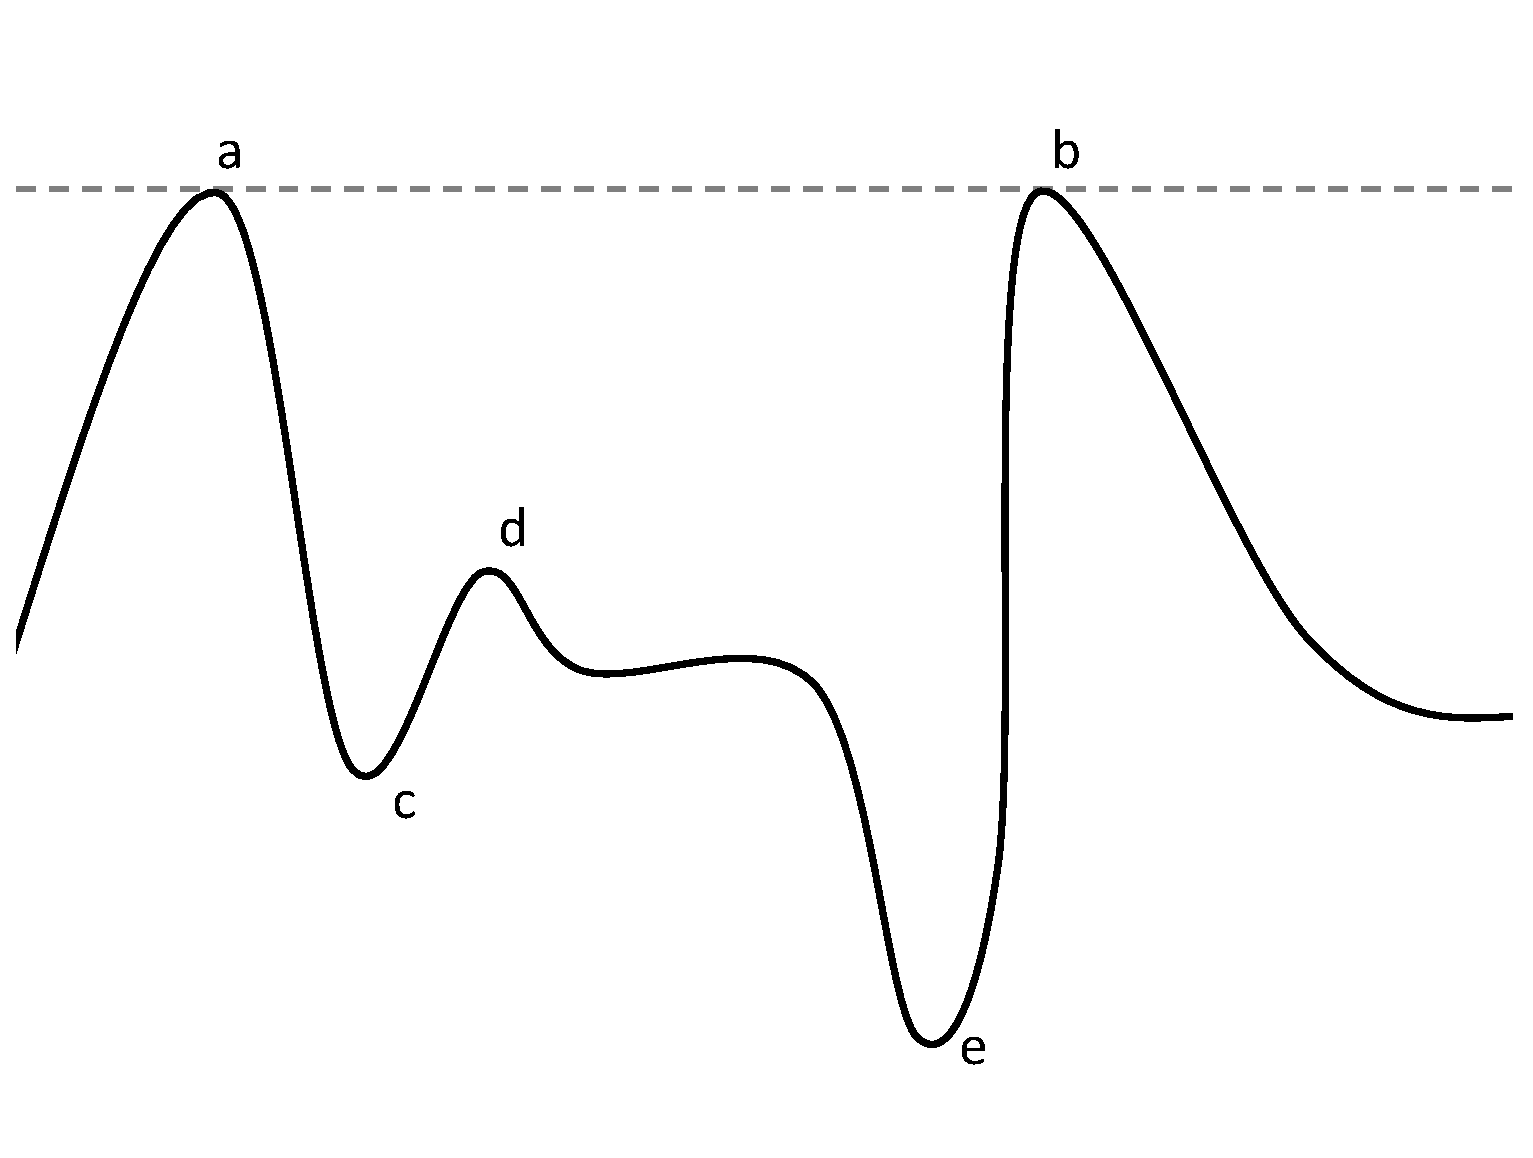
\includegraphics[width=0.6\paperwidth]{searchSpace}
\caption{Examples of local and global optimums.}
\label{localAndGlobalOptims}
\end{figure}


In \ref{localAndGlobalOptims}, we can see different examples of global and local optimums. The points labeled \emph{a} and \emph{b} are both global maximums, as they have the same value. The points
\emph{c} and \emph{d} are respectively local minimum and maximum, while \emph{e} is the global minimum.

A formal definition of the most simple and generic optimization problem would be:

\begin{equation}
min\, f(x)\, s.t.\,(x\in X)
\end{equation}

Where \emph{X} is our search space and \emph{f(x)} the objective function we want to minimize. 

\subsubsection{No Free Lunch Theorem}

\subsubsection{Combinatorial Optimization}

\subsection{Numerical Optimization}
\subsubsection{Linear Programming}
\subsubsection{Quadratic Programming}
\subsection{Nonlinear Programming}

\subsection{Multi-Objective Optimization}

Multi-objective optimization (also called multi-criteria optimization), or MOO, departs significantly from previous categories of optimization in the fact that you have to consider multiple objective functions instead of one. A main aspect of MOO is the way to conciliate these objectives, which are usually contradictory.
An example of real-world everyday MOO problem could be choosing the mean of transportation for a travel, trying to find a balance between speed and cost. Airplane is the fastest way of transportation, but is expensive. While car is slower, it is cheaper. Train is slower than plane, more expensive than car, but can preferred as the best compromise. There still, however, are solutions which are strictly worse than others (in our example, renting an helicopter would probably be both more expensive and slower than buying a seat on a commercial airplane).
From this example, we can see that, for a MOO problem, there rarely is a clear-cut "best" solution. And, more importantly, that even some solutions which are not optimum for \emph{any} of the objectives can be deemed satisfying. 


[[FORMULATION OF A MOO PROBLEM]]

We will now see which strategies have been proposed to deal with such a type of problem.

\subsubsection{Objectives Aggregation}

The first approach is to transform the MOO problem back to a mono-objective optimization problem, by aggregating the different objectives into one.

[[Different strategies : pondered mean, goal programming, min-max -> See thesis JB Welcomme for ref]]

Whatever the chosen aggregation strategy will be, this approach presents severe limitations. 

\subsubsection{Pareto Dominance}

\subsubsection{\emph{A priory} versus \emph{a posteriori} approaches}

\subsection{Multidisciplinary Optimization}

\subsection{Optimization under Uncertainties}

\subsection{Optimization in Dynamic Environments}

\subsubsection{Genetic Algorithms}


\end{document}


\part{Multi-Agents Systems and AMAS Theory}

[[NO CHAPTER ??]

As we said at the end of the last part, providing a method able to scale to the needs of the full range of optimization problems would require to it to be capable of adapting itself to the problem at hand.
The main theme of the SMAC team\footnote{\emph{Systèmes Multi-Agents Coopératifs} (Cooperative Multi-Agents Systems)}, in which this thesis has been realized, in the Adaptive Multi-Agent Systems (AMAS) Theory. This theory relates to the design of agent-based complex systems with self-adaptive capabilities.

In this part we will present first a short history of multi-agents systems, before concentrating on the concepts of the AMAS theory.

\section{Multi-Agents Systems}

Multi-Agents Systems (MAS) are a relatively recent field which can be seen as the intersection of Artificial Intelligence (AI) and Systems Theory. As a reminder, the AI field was developed in 1950s as "the science and engineering of making intelligent machines." [[source MacCarthy cf wikipedia]] This rather ambitious project was somewhat toned down during the 70s when the field was the subject of several setbacks leading to an "AI winter"[[REF ? Russell and Norvig ?]], which effects can still be felt today. The commonly accepted reason for this setback was that the researchers have been too much ambitious in their expectations of the breakthroughs which would be produced by the field, and did not take enough into account the inherent complexity of some of the task they were proposing to handle (\emph{e.g. language processing}).

[[TO PUT? Several specific subfield subfields of AI have been defined, among which we can find automated problem solving, machine learning, robotics, knowledge engineering, planning, affective computing \emph{etc.}]]

This disgrace period of the IA field ended with the success of expert systems in the 80s. These systems aim to emulate the ability of a human being to take decisions based on expert knowledge, using inference mechanisms (via an \emph{inference engine}) and a rules database.
However, even expert systems cannot avoid the complexity of modeling knowledge, and are still ultimately limited by the growth of their rules database. This concern, among others (such as privacy of informations) lead to a new field of IA named Distributed Artificial Intelligence (DAI)[[REF?]], where several expert systems collaborate to provide a collective diagnostic of a situation.

In parallel to the developments of AI, another field of knowledge emerged in the beginning of the century, Cybernetics (also called System Theory), the study of self-regulating systems. Interestingly, this field had radically different origins from AI, taking root in social and natural sciences. These two disciplines had a somewhat uneasy coexistence for some times during the 50s, after which AI took the lead and cybernetics[[see on the importance of being emergent - Peter Cariani]].The field knew a revival in the 70s with the "new cybernetics", or "second-order cybernetics", which introduces the study of self-organizing systems and the notion of observer.

It is interesting to note the conflicting nature of AI and cybernetics. AI initially based itself on a reductionist approach of knowledge, using symbol manipulation coming from algebra and logics. Cybernetics was part of the more general [[epistemic/epistemological ??]] upheaval of constructivism.

It is a the conjunction of these two seemingly contradictory fields that was born the study of Multi-Agents Systems.

\subsection{Principles of Multi-Agents Systems}

Before talking about Multi-Agents Systems (MAS), we must explain the notion of \emph{agent}. Several conflicting definitions of what is an agent have been proposed. We keep here the (mostly) consensual one proposed by Wooldridge in \cite{wei1999mutiagent}:

\definition{Agent}{"An \emph{agent} is a computer system that is \emph{situated} in some \emph{environment}, and that is capable of \emph{autonomous action} in this environment in order to meet its design objectives."}

Based on this definition, a MAS is a system composed of several agents, interacting among each other and with their environment.

The \emph{autonomy} of an agent is the fundamental characteristic which differentiates it from, for example, the concept of object. While an object is a passive entity encapsulating some data and functions, waiting to be solicited, an agent is capable of acting and reacting to changes in its environment. From this comparison it should be clear that the concept of agent is, like the concept of object, the building brick of a paradigm which can be used to model a complex reality. And indeed, agents have been used in a great variety of fields, a fact which can contribute to explaining the difficulty to produce an unified definition of the concept.

\subsection{Self-* capabilities}

While it is not true for all MAS, some interesting properties can be achieved when taking advantage of the autonomy of the agents. This autonomy, coupled with an adequate behavior of the agents, can lead to systems which are able to adjust, organize, react to changes \emph{etc.} without the need for an external authority to guide them. These properties are regrouped under the term self-* capabilities (self-\emph{tuning}, self-\emph{organizing}, self-\emph{steering} ...).

Not all MAS necessarily present all of these self-* capabilities, but, as a result of building a system from autonomous and locally situated agents, many MAS will exhibit them to some degree. Consequently, MAS are often very good at dynamically taking into account changes into their environment. For example, a multi-agent system in charge of regulating the traffic of packets in a network could be able to react efficiently to the disappearance of some of the relay nodes.

\subsection{Multi-Agents Systems for Distributed Problem Solving}

In the context of this thesis, we will concentrate on the application of MAS in the specific context of distributed problem solving (DPS). However it can be useful to bear in mind the others possibles application fields: social simulation, biological modeling, systems control, robotics \emph{etc.} and agent-oriented modeling as a programming paradigm in general.

\subsubsection{Multi-Agents Systems for Combinatorial Optimization}

[[TODO: CITER TRAVAUX IIIA]]

The major part of the literature on the application of MAS to \emph{combinatorial} optimization, mainly in the context of DPS concerns Distributed Constraint Satisfaction Problems (DCSP, or DisCSP) and their extension, Distributed Constrained Optimization Problems (DCOP, or DisCOP).

DCSP is a formalism to model Constraint Satisfactions Problems (CSP) using agents. A CSP is defined as a triplet <$X,D,C$> where:
\begin{compactitem}
\item $X = {x_1, ..., x_n}$ is the set of variables.
\item $D = {D_1, ..., D_n}$ where $D_i$ is the definition domain of $x_i$.
\item $C ={c_1, ..., c_m}$ the set of constraints to satisfy.
\end{compactitem}

The goal is to find an assignment to the set of variables $X$ which:
\begin{compactitem}
\item comply with their definition domains $D$.
\item satisfy the set of constraints $C$.
\end{compactitem}

In general, CSP are NP-complete[[REF?]].

Usually, the constraints of a CSP are binary. In this case, the CSP can be represented as a graph for which each vertex is a variable and each constraint an edge.

\begin{figure}[]
\centering
	\begin{subfigure}[b]{0.35\textwidth}
			$X = \{x1, x2, x3\}$\\
			$D = \{\{0,1\}, \{1,2\}, \{0,1,2\}\}$\\
			$C = \{(x1 \neq x3), (x2 \neq x3)\}$		
		\caption{formal definition.}
	\end{subfigure}
	\begin{subfigure}[b]{0.45\textwidth}
			\centering
			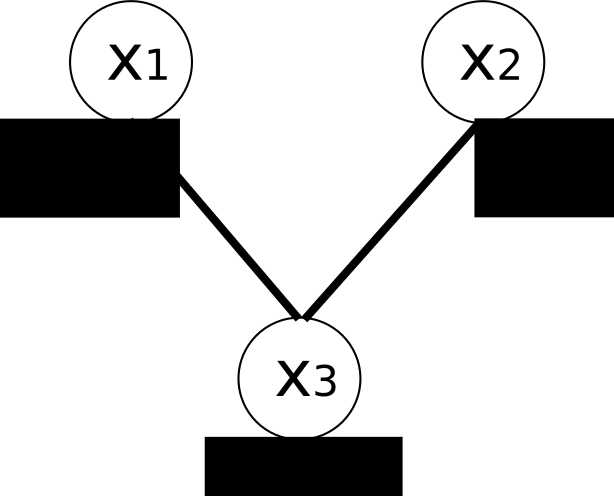
\includegraphics[width=0.7\textwidth]{DCSP}
			\caption{corresponding agent graph.}\label{dcsp:graph}
	\end{subfigure}

\caption{An example of DCSP representation.}
\label{dcsp}

\end{figure}

From this graph representation, the DCSP formalism\cite{yokoo1998distributed} models a CSP  as an agent graph, with each agent in charge of assigning a value to a variable based on local and shared constraints. A DCSP is described as a quadruplet <$X, D, C, A$>. $X, D$ and $C$ have the same meaning than in the CSP formalism, while $A$ is the set of agents. For each each agent in $A$ has the responsibility of a subset of $X$ and knows the constraints related to the variables in its care. The most common assumption is that each agent has the responsibility for one and only one variable. See \figurename{} \ref{dcsp} for an illustration of the graph transformation of a DCSP.

One classical example of DCSP solver is Asynchronous Backtracking (ABT)[[REF: M. Yokoo. Distributed Constraint Satisfaction: Foundation of Cooperation in Multi-agent Systems. Springer, 2001.]]. ABT creates a total ordering on the agents and models the relations between agents as directed links, in order to make the network cycle-free. In ABT agents exchange \emph{nogoods}, which are conditional constraints (the constraint is valid as long as some other agents do not change states). When an agent detects a no-good, it checks if it can change its state in order to solve it. If it is possible it does so and informs the agents it is linked to. Else it propagate it to the lowest priority agent its known (based on the ordering) involved in the no-good, creating new links if necessary.

An extension of DCSP has been proposed for formalizing Distributed Constrained Optimization Problems (DCOP, or DisCOP). DCOP is to COP the equivalent of DCSP to CSP. While a DCOP is described in the same way than a DCSP, the semantic and goal are different.
In DCOP, the constraints in $C$ represent a decomposition of a global cost function, which the agents try to minimize (or alternatively, maximize). Each constraint is now seen as a local cost function giving the cost associated with each state of two variables (in the context of DCOP, the term \emph{constraint} is sometimes replaced by the terms \emph{cost function} or \emph{soft constraint}). Formally, DCOP consider the global objective-function $F(X) = \sum_{x_i, x_j \in X} c_{ij}(x_i,x_j)$ where $c_{ij}$ is a local cost function associated with the states of $x_i$ and $x_j$.

A classical use of DCOP is unsolvable CSP, that is problems where there is no solution which satisfy all the constraints. In these cases the problem can be changed into a DCOP with the new objective to minimize the number of violated constraints. If we wanted to transform the problem shown in \figurename{} \ref{dcsp} (ignoring the fact that this DCSP is in itself solvable), we could replace the constraints in $C$ by the function $c_{13}$ and $c_{23}$ defined as follow:

\begin{center}
\begin{tabular}{ccc}
\textbf{$x_1$}	& \textbf{$x_3$} & \textbf{$c_{13}(x_1,x_3)$}\\
\hline
0   & 0	& 1\\
\hline
1   & 0	& 0\\
\hline
0   & 1	& 0\\
\hline
1   & 1	& 1\\
\hline
0   & 2	& 0\\
\hline
1   & 2	& 0\\
\end{tabular}
\quad
\begin{tabular}{ccc}
\textbf{$x_2$}	& \textbf{$x_3$} & \textbf{$c_{23}(x_2,x_3)$}\\
\hline
1   & 0	& 0\\
\hline
2   & 0	& 0\\
\hline
1   & 1	& 1\\
\hline
2   & 1	& 0\\
\hline
1   & 2	& 0\\
\hline
2   & 2	& 1\\
\end{tabular}
\end{center}

In the context of this framework, many techniques have been proposed. One of leading algorithms to date is the Asynchronous Distributed Optimization Algorithm (ADOPT)[[REF]].In order to work, ADOPT needs to reformulate the problem by introducing a total ordering on the agents. This ordering allows to create a tree representation of the problem, where each agent has a single parent and multiple children. The algorithm in itself is articulated on two main ideas:

\begin{compactitem}
\item each agent asynchronously changes states when it perceives a possible better solution.
\item the agents can backtrack to previously explored solutions, but only if this current state is worse than a specific \emph{backtrack threshold} determined by its parent agent.
\end{compactitem}

Another well-known algorithm is Optimal Asynchronous Partial Overlay (OptAPO)[[REF]]. this algorithm is an adaptation of Asynchronous Partial Overlay (APO), which was proposed for solving DCSP. OptAPO, as APO, is based on the principle of \emph{Cooperative Mediation}, where the agents try to identify parts of the problems which can be solved in a centralized way (using centralized solvers such as Branch-and-Bound). During solving, some of the agents take the role of mediator during \emph{mediator sessions}, where they compute a solution to a part of the whole problem and propose solution to the others agents involved into the mediation.

The DCOP formalism is very popular in its own right as it allows a clear framework on how to represent this type combinatorial problems without putting too much restriction on how the problem  is solved. The exact information shared by the agents, and the way they communicate among themselves is not constrained. However this formalism is not without limitations.\\
While some works successfully used DCOP in the context of continuous optimization\cite{stranders2009decentralised}, this formalism is not adequate to handle the full range of problems we would like to consider here. DCOP was conceived for a specific type of problems where the difficulty resides in the combination of multiple constraints. These problems are supposed to be easily decomposable into several cost functions, where the cost values associated to the variables states are supposed to be known. This major assumption does not stand for complex continuous optimization problems (such as MDO problems for example), where the complexity of the models and their interdependencies cause this information to be unavailable in most cases. Modeling such problems with DCOP would be impossible in most case, as most agents would potentially be related to every other agent and the cost functions would be unknown.

One a side note, it is interesting to note that many methods require non-trivial changes to the topology of the agent graph to work (acyclic graph, tree structure ...), both in the context of DCSP and DCOP. These changes can  be potentially extensive operations in themselves, and must be applied carefully lest the relevance of the result be compromised. Consequently, existing agent-based optimization techniques for DCOP may require a strong expertise to be efficiently applied\cite{Ka2011.6}.

\subsubsection{Multi-Agents Systems for Continuous Optimization}

[[Signaler PSO ?]]

While MAS are a very popular approach for solving combinatorial optimization problems, their application to continuous optimization problems is scarce at best. One could explain this discrepancy by the fact that continuous optimization problems are in general more difficult to decompose than combinatorial ones.

As said in the previous section, an adaptation of DCOP with continous variables has been proposed in \cite{stranders2009decentralised}. This work proposes an adaptation of the max-sum algorithm in the continuous case by redefining the two operations of summation and maximization in order to be able to use them over continuous utility functions.
However, this work concentrates on a specific type of problem (distributed sensor networks) and the utility functions must be piecewise linear. It is not applicable to broader scope of continuous optimization problems which concern us here.

A notable work on the subject of general continuous optimization is the MASCODE algorithm \cite{welcomme2006self}, which concentrates on MOO and MDO problems. In MASCODE, each agent in in charge of a discipline and the links between agents represent the dependencies between the different disciplines. For each input of a discipline, a \emph{physical validity interval} and an \emph{objective validity interval} are defined. These two intervals represent respectively the physical constraints of the model and the boundaries of an objective to achieve. Using these two measures, a satisfaction measure is defined using a parametric piecewise continuous function. The basic idead of this satisfaction measure is as follows: 
\begin{compactitem}
\item when the value of the input is in the boundaries of the objective validity interval, the satisfaction of the agent regarding this input is high,
\item when the value of the input is outside of the objective validity interval but inside the physical validity interval, the satisfaction lower,
\item if the value of the input goes outside the physical validity interval, the satisfaction becomes minimal.
\end{compactitem}

The agents use the values of their inputs to send \emph{forward messages}, informing others agents of the values of their outputs. Upon reception of these messages, one agent use these new values to recalculate its own outputs (potentially sending in turn new \emph{forward messages}) and send \emph{backward messages} to the agents controlling their inputs. These \emph{backward messages} are modification requests indicating the satisfaction of the requesting agent. Upon reception of such messages, the agent will select which ones to handle based on the current satisfaction degree of their emitter and will change the value of its inputs accordingly (sending in its turn new \emph{backward messages} if required).

This algorithm is very interesting as it make very few presupposition concerning the shape of the optimization problem. The problem can be expressed as initially conceived by the designer, without requiring special transformation operations. Still, there is some limitation to the expressiveness of the formulation. The possibilities for the designer to express constraints and objectives on the problem are restricted to the specific use of the physical and objective validity intervals. As a consequence, constraints and objectives cannot be expressed independently, and can only concern \emph{one} variable at a time. While this latter limitation can somewhat be circumvented by introducing artificial disciplines placeholders, the natural modeling of the domain is then lost. This limitation can be explained as a consequence to the specific application domain which was considered for the algorithm (industrial product design)

[[dire qu'on va s'inspirer de MASCODE dans notre algo de résolution (mais pas pour NDMO => peut être le dire dans la partie sur le SMA en lui-même)]]

\subsubsection{Analysis of Multi-Agent Systems for Distributed Problem Solving}

We have seen in this section how MAS have been applied for problem solving. While the solving of discrete constraint satisfaction and optimization problems has been a very popular topic of interest, very few works exist concerning the solving of continuous problems. Among the few existing works, most concentrate on specific application topics, thus no real unified effort exist in this regard comparable to one which can be observed for discrete optimization.
[[EXPAND ??]]

\section{The Adaptive Multi-Agents Systems Theory}

\subsection{Theorem of Functional Adequacy}

The conception of MAS for problem solving is not an easy endeavor. Suffice to observe that most of the multi-agents systems algorithms dedicated to problem solving proposed by the scientific community are nature-inspired (ants, flocks, bees, bats etc.). Indeed, Nature had a long time to experiment on several arduous problem and a lost of subjects at hand. Why would we not take advantage of that? However, such a strategy presents a severe limitation, as it can bring us existing solutions to apply to potential problems, but ultimately cannot help us to find potential solution to some existing problems. By restricting ourself to nature-inspired mechanisms we are bound to their application field.\\
The inspiration for things such as the internal combustion engine was not found in nature, since no other biological organism than men ever bothered with something in appearance so foolish as trying to reach for the Moon\footnote{In total honesty, it is possible that some other organisms already tried to reach for the Moon. But it seems such behavior did not give them enough significant evolutionary advantage to be noteworthy (except of course for a specific cow in the popular nursery rhyme [[put a ref ?]]).}.

In order to overcome this limitation, we need to rely on a more theoretical approach which would help us in the conception of MAS for which we do not know any existing applicable mechanisms. Such an approach is provided by the Adaptive Multi-Agents Systems (AMAS) theory.

The AMAS theory was developed by the SMAC team and formalized in \cite{glize2001adaptation}. It focuses on cooperation as the fundamental mechanism of MAS design.

At the basis of the theory is the modeling of a system as a set of entities, the agents, interacting with each others and with their environment. This modeling is holonic[[?]] at its core, since the agents themselves can also be viewed as systems for which the environment consists of the other agents and the environment of the encompassing system.

The system can be deemed to be \emph{functionally adequate} by an external observer if this latter judges that the system as a whole correctly accomplishes its function in regard of the environment. This external observer can be considered to be a perfect oracle, in a way similar to the Laplace's demon, knowing exactly which will be the consequences of each interactions between the system and its environment\footnote{It is important to understand that, from a theoretical point of view, the notion of functional adequacy is inherently subjective, and depends on the observer. In practice it is however usually more easier to attain a reasonable consensus. For example a natural system will usually be deemed adequate if it survives and thrives in a sustainable way. For an artificial system it is often even easier since the functional adequacy correspond to the function expected by the designer of the system.}.

The AMAS theory identifies three categories of interactions between a system and its environment:
\begin{compactitem}
\item Cooperative action: the acting entity is beneficial to the other.
\item Antinomic action: the acting entity is detrimental to the other.
\item Neutral action: the acting entity has no effect on the other.
\end{compactitem}

From this categorization, the theory draws its formal definition (and fundamental axiom) of functional adequacy:

\definition{Axiom of functional adequacy}{A functionally adequate system has no antinomic interaction with its environment}

\begin{figure}
\centering

	\begin{subfigure}[b]{0.45\textwidth}
		\centering
		\includegraphics[width=\textwidth]{system_non_adequate}
		\caption{system not functionally adequate.}
	\end{subfigure}
	\hfill
	\begin{subfigure}[b]{0.45\textwidth}
		\centering
		\includegraphics[width=\textwidth]{system_adequate}
		\caption{functionally adequate system.}
	\end{subfigure}
	
\caption{Comparison of a system not functionally adequate and a functionally adequate one.}
\label{adequacy_comp}
\end{figure}

An illustration this axiom is shown on \figurename{} \ref{adequacy_comp}.

%\definition{Internal cooperative medium system}{A system in which the agents only have cooperative interactions with each others or their environment[[?]]}

Using this axiom, several properties has been demonstrated concerning a specific set of \emph{internal cooperative medium systems}, defined as systems in which the agents do not have any antinomic or neutral interaction (illustrated on \figurename{} \ref{internal_cooperative_comp}). We will not enter here in the details of these properties and their demonstration
, the interested reader can refers to [[REF]]. Suffice to say that these properties lead to the central theorem of functional adequacy:

\definition{Theorem of Functional Adequacy}{For each functionally adequate system there exists a internal cooperative medium system also functionally adequate in the same environment}

\begin{figure}
\centering

	\begin{subfigure}[b]{0.35\textwidth}
		\centering
		\includegraphics[width=\textwidth]{system_non_cooperative}
		\caption{system which does not have an internal cooperative medium.}
	\end{subfigure}
	\hfill
	\begin{subfigure}[b]{0.35\textwidth}
		\centering
		\includegraphics[width=\textwidth]{system_cooperative}
		\caption{internal cooperative medium system.}
	\end{subfigure}
	
\caption{Illustration of internal cooperative medium system.}
\label{internal_cooperative_comp}
\end{figure}

This theorem is at the core of the AMAS approach of system design. We already know that for each problem there is possibly an infinity of equivalent systems producing the same adequate functioning. Using the theorem of functional adequacy we can concentrate on designing an internal cooperative medium system, that is, designing a system were the agents cooperate among themselves and with their environment. The goal of a designer using this approach is thus to study the nature of the interactions between the entities of the problem domain, and to see how the non-cooperatives situations could be corrected in order to obtain an internal cooperative medium system.

In addition to providing us with a theoretical context, this approach gives us another interesting property: as the design of the system is focused on the local interactions of the agents, we do not need to explicitly take into account the global function of the system. This property is extremely significant. If the global function is complex, it can be extremely difficult to successfully design a system which explicitly tries to achieve the global function (top-down approach). By concentrating on the local functions of the agents, we can spread the complexity and ease the design of the system (bottom-up approach). [[PARLER D'EMERGENCE ? SI OUI QUAND ? => Après le fonctionnement du système ?]]

\subsection{Cooperative Agents and Non Cooperative Situations}

To guide the designer during the building of such a internal cooperative medium system, the conditions of what make an agent a \emph{cooperative agent} have been further formalized. An agent is said to be cooperative if it satisfies three conditions:
\begin{compactitem}
\item $C_{perception}$ Every perceived signal can be understood without ambiguity
\item $C_{decision}$ Every interpretation must produces useful information
\item $C_{action}$ Every action done based on the decision must be useful
\end{compactitem}

Based on these condition, a set of \emph{Non Cooperative Situations}(NCS) has been identified. These NCS correspond to interactions which are not cooperative and must be removed for the system to be an internal cooperative medium system. The NCS are classified based on the condition they violate. The table in \figurename{} \ref{NCS} shows this classification.

\begin{figure}
\centering
\begin{tabular}{|c|c|}
\hline
\textbf{Violated condition}	& \textbf{Corresponding NCS} \\
\hline
$C_{perception}$     & Incomprehension, Ambiguity     \\
\hline
$C_{decision}$      & Incompetence, Unproductiveness[[?]] \\
\hline
$C_{action}$     & Uselessness, Competition, Conflict\\
\hline
\end{tabular}
\caption{The conditions for cooperation and corresponding NCS}
\label{NCS}
\end{figure}

The different NCS are:

\definition{Incomprehension}{The agent is not able to extract information from a received message.}
\definition{Ambiguity} {The exact meaning of a message cannot be determined, or lacks required informations.}
\definition{Incompetence}{The agent does not have the capabilities to handle a received information.}
\definition{Unproductiveness[[?]]}{A received information does not lead to any useful conclusion.}
\definition{Conflict}{The action of the agent is incompatible with an action from its environment.}
\definition{Competition}{The action of the agent leads to the same result than an action from its environment.}
\definition{Uselessness}{The action of the agent has no effect on itself or its environment.}

A cooperative agent actively tries to avoid these NCS and, should this fail, to solve them to the best of its capabilities. To this end, three distinct mechanisms can be used\cite{bonjean2009engineering}:

\definition{1. Tuning}{The agent can change one or several of its internal parameters (\textit{e.g.}, adjusting the priorities of its behavior rules)}
\definition{2. Reorganization}{The agent can change its relationship with its environment (\textit{e.g.}, removing or creating new links with others agents)}
\definition{3. Evolution}{The agent can change the nature of its environment (\textit{e.g.}, removing or creating new agents)}

The order of these mechanisms usually correspond to their level of disruption (\textit{i.e.}, adjusting its parameters usually has less consequences than creating and removing agents). In general, it is preferable to make the less disruptive possible adjustment. One can for example design the agents based on an escalation principle, where the agents try to solve NCS first by using tuning, escalating to a more disruptive mechanism only when the previous ones failed to solve the NCS. Of course, a NCS situation being by itself disruptive, it is sometime more efficient to immediately make a more radical adjustment in order to solve the NCS more quickly. The designer will have to balance these concerns according to the specificities of the system.

\subsection{The Importance of Locality}
[[Explain how locality is important to scale to big problems and in the concept of emergence => To put in the section A Multi-Agent System for Optimization ??]]

\subsection{ADELFE - A Method for Designing AMAS} 
[[TODO ? AND MAY ? HERE OR IN THE IMPLEMENTATION PART ?]]

[[Quand je parle d'ADELFE, signaler l'existance d'autres méthodes existantes. Expliquer que ces méthodes sont génériques et ne dispensent pas d'un gros travail d'expertise.]]

\subsection{Conclusion on the Adaptive Multi-Agents Systems Theory}

We presented here the AMAS theory. This theory presents a way to models systems by their interactions with their environment and identify the special category of internal cooperative medium systems.

An interesting aspect of this theory  is that it provides a guidance to build a multi-agent system based on the problem to solve. Classical solving methods often use a very rigid formalism which needs to be followed. For example, genetic algorithms are a very powerful technique, but they require the problem to fit the genetic representation/fitness function model. To use these kinds of methods, one would now be presented to a whole new problem: "how to express my problem to fit the solution I want to employ ?"

[[These methods can be said to be "solutions looking for problems"]]

While a non-negligible part of real-world problems are more or less straightforwardly translated in such formalisms, there is still a whole range of problems for which this translation is not so easy. This can be either because no method adequate enough for the domain was proposed, or because there is no consensual representation of the domain. For these problems, the AMAS theory can provides an interesting asset as the design of the MAS is based on the problem domain. The solution is adapted to the problem, instead of requiring the problem to be adapted to the solution.

We can say that, while the AMAS approach can be applied to any kind of problem, it seems to be especially adequate when trying to solve problems which are still in an exploratory phase, where no "clear-cut" solution exists.




\part{A Multi-Agent System for Optimization}

\chapter{Agent-Based Modeling of an Optimization Problem}

\chapter{Simulation Rules}

\chapter[Solving Rules}

\chapter[Agent Architecture}

\chapter{Analysis - Collective Solving Patterns}

\part{Design, Implementation and Contribution Toward AMAS4Opt}

One of our concerns was not only to propose a new approach for continuous optimization, but also to put this approach in practice by integrating it into a proof-of-concept prototype. To this end we worked with domain specialists and software development experts to propose such a tool, basing ourselves upon the ADELFE method. This method aims to guide the development of AMAS-based softwares from high level user requirements to the implementation nuts and bolts. Using ADELFE we made a formal analysis of the domain and actor involved in the use of such tool.

We also use the design tools developed in conjunction with the method to instantiate our MAS with the final end to integrate it with a functional end-user interface. Notably, the recent MAY framework, which was developed in order to provide suitable abstractions as well as reusable software components for the development of agents and multi-agents systems. We contributed to the enrichment of its component library by developing a a general and modular agent architecture consistent with the AMAS theory, in particular by proposing a modular skill stack principle, where different skills can be composed to address specific requirements.

While such work could seems to concerns more software engineering experts than computer scientists, we will see how existing MAS oriented methods such as ADELFE are still too broad level to be successfully directly applied to any domain (and more so to continuous optimization) without an important agent expertise and extensive research work. We will detail how the scientific work we produced and presented in the previous part, especially the identification of various NCS and the mechanisms to solve them, can be generalized into \enquotes{building blocks}. These building blocks could be then reused to guide the conception of other MAS for the domain of problem solving. This work places itself into a more general effort to provide a general reusable toolbox for assisting non experts in applying AMAS to the domain of optimization, under the name \emph{AMAS4Opt} (AMAS for Optimization).

\chapter{ADELFE}

\section{Overview of ADELFE}

In section \ref{AMAS-ADELFE}, we succinctly presented ADELFE\footnote{\url{http:/www.irit.fr/ADELFE/}}, the method which has been proposed for the design of AMAS. In this chapter we get back in more details about this method and what benefits it provided for the design of our system. 

ADELFE is a method devoted to software engineering of adaptive multi-agent systems, developed by ARTAL and IRIT and founded by the RNTL 2000 program. The name “ADELFE” is the French acronym for "toolkit to develop software with emergent functionality" (Atelier pour le DEveloppement de Logiciels à Fonctionnalité Emergente.

The ADELFE method in itself is based the Rational Unifed Process (RUP) and is defined following the Software Process Engineering Meta-Model (SPEM)  \cite{bernon2003adelfe,picard04phdthesis}. Since its revision \cite{Ro2008.3}, it is composed of five \emph{Work Definitions} ($WD$), themselves decomposed in several \emph{activities} making use of UML as well as the AMAS-ML and muADL languages. An overview of the method is shown on \figurename{} \ref{ADELFE_phases}.

\begin{figure}
\includegraphics[width=\textwidth]{AdelfePhases}
\caption{Overview of the ADELFE Method}\label{ADELFE_phases}
\end{figure}

In regard of the RUP, ADELFE adds specific activities and roles which are specific to its approach for the design of AMAS.\\
The final requirement study ($WD_2$), was complemented with activities 6 and 7-2 concerning the characterization of the system environment and the identification of cooperation failures during the determining of the use cases.During the Analysis ($WD_3$), additional activities 11 and 12 respectively check for the adequacy of AMAS to the problem and identify the agents involved in the system being built, while activity 13 is complemented with a step concerning the study of the relationships between agents. During the design ($WD_4$), activities 15 et 16 concerns the design of the system and the agents, while activity 17 concerning fast prototyping was added in order to be able to quickly test the proposed behavior of the agents. The development phase ($WD5$), which was not present in the initial version of ADELFE, concerns the architecture and the implementation of the agents and the system.

\section{Applying ADELFE for the Design of a Continuous Optimization Tool}

Based on the guidelines of the ADELFE methodology we defined the requirements of the tool we proposed to develop. The following functionalities were identified:
\begin{compactitem}
\item Our tool will allows users to solve multidisciplinary optimization problems.
\item  The user will be able to load disciplinary models into the tool, express some constraints and objectives on these models and then use and interact with the tool to solve the defined problem.
\item Our tool will be reusable from one optimization problem to another in different application domains and will be a generic tool.
\item The user will be able to specify a specific resolution process to be used, but it will not be mandatory.
\item The user will be able to load into the tool different models of the same discipline (i.e. aerodynamics, acoustics ...), but with a different fidelity. It will be possible for the user to specify the tool to take in account these different models during the problem solving.
\item The user will be able to express uncertainties on some part of the models or input variables.
\item The resolution will take into account these uncertainties.
\item The tool will be able to integrate some well-known optimization techniques, and will allow the user to add new techniques to use during solving. The tool will also be able to interact with others optimization tools to ease the optimization process.

\item The user will be able (at runtime):
	\begin{compactitem}
    \item to monitor the system activity,
    \item to observe time history qualitative indicators,
    \item to adjust its parameters.
    \end{compactitem}
\end{compactitem}

\begin{figure}
\includegraphics[width= \textwidth]{Use_cases}
\caption{Actors and use cases identified during requirements studies}\label{Use_cases}
\end{figure}

Several entities interacting with the tool were also identified. The \emph{Method expert} adds new optimization methods into the system. The expert field can be optimization methods (classic methods, AMAS methods ...) or uncertainties. The \emph{Model expert} adds new models into the system. The role of the \emph{Engineer} is to use the different elements defined by the other experts to define new problem for the system to solve and to monitor the functioning of the system. At last, the \emph{AMAS expert} has to define and tune the agents of the system. The system should also be able to integrate with external optimization and modeling tool, in order to accommodate the existing workflow and constraints of the users.

The different use cases which were identified for each of these entities are presented in \figurename{} \ref{Use_cases}.

\chapter{MAY Architecture}

[[First generic AMAS architecture ??]]

To implement the MAS, we used the Make Agents Yourself (MAY) framework. MAY is a component-based framework which automatically generate an implementation of an agent architecture from a given description.

[[PROVIDE SOME REF -> ASK VICTOR -> his phd \cite{No2012.2}]]

The Adelfe methodology proposes an abstract agent architecture (represented in \fig{[[TODO]]}), which we translated into the MAY architecture description language, SpeADL. [[As our agents only act and communicate using message-passing, we could make some simplification concerning the modeling of the communication and action capabilities.]]
All our agents use the same AMAS architecture. They are differentiated by specific implementations of the components. For example, \emph{Model} and \emph{Variable} agents will have different implementations of the \emph{Behavior} component.

For the sake of clarity, the agent architecture is separated in three views: the \emph{behavior}, \emph{communication} and \emph{monitoring} views.

\subsection{Behavior}

The \emph{behavior} view (\figurename{} \ref{Arch-behavior}) contains the components related to the behavior of the agent. 

\begin{figure}
\centering
\includegraphics[width=0.6\paperwidth]{ID4CS_Speadl_behav}
\caption{Agent Architecture - Behavior view.}
\label{Arch-behavior}
\end{figure}

The \emph{Behavior} component contains the rules which dictate the behavior of the agent. This component can be seen as the [[chef d'orchestre]] of the architecture. This component exposes to the outside of the environment the \emph{Step} port, which is used to make the agent execute a step. During a step the \emph{Behavior} component executes the agent rules. These rules will in return make use of the others components of the agent.

[[DIRE QUE LES RULES ONT ETE PRESENTEES DANS UN CHAPITRE PRECEDENT]]

The \emph{State Vault} contains the state of the agent. It is used by the components which need to save and read some state variables. Centralizing all the states variables into one component provides several benefits. First it is easier to save and restore the state of the agent, as we just need to save the content of the vault. It is also simple to share some data between components, as long as these components have access to the vault. And it is easy to provide a view of the agent state by just reading the State Vault.
This approach has however several drawbacks. It adds some boilerplate code when writing code using the agent state, as we need to explicitly read the value from the vault (and possibly store it to the vault if modified). It make more difficult to track side-effects, as it is not obvious to know which component uses which value. At last there is no way to strictly enforce that components only use the State Vault for storing state values, as neither Java nor MAY can provide such guarantee.

The \emph{Skills} component contains the skills of the agents. Skills are [[skill definition]]. Each agent type has its own skills set, and skills can require to read and modify the agent state (thus the link between this component and the \emph{State Vault}).
Some skills are used directly from the \emph{Behavior} rules but some skills can also be used by others skills.
Some examples of skills are: for a \emph{Variable agent}, the capability to change its value based on the requests it received and its old value. For a model agent, the capability to translate a request it received to change one of its outputs into a set of requests to send to its inputs.

[[PARLER DU FAIT QUE LES SKILLS ONT LEUR PROPRE ARCHITECTURE ??]]

The \emph{Aptitudes} component contains the aptitudes accessible to the agents. Aptitudes are [[Aptitude definition]]. Unlike skills, aptitudes are general capabilities which do not rely on the state of the agent. Consequently, all agent types have access to the same aptitudes, and there is only one implementation of the \emph{Aptitudes} component.
Some aptitudes are used directly from the \emph{Behavior} rules but some aptitudes can also be used by skills or others aptitudes.
Some examples of aptitudes are: ordering a set of requests from the most to the least important. Make some manipulations on the exchanged values (adding, calculate the norm etc.).

\subsection{Communication}

The \emph{communication} view (\figurename{} \ref{Arch-comm}) presents the components related to the communication capabilities of the agent. 

\begin{figure}
\centering
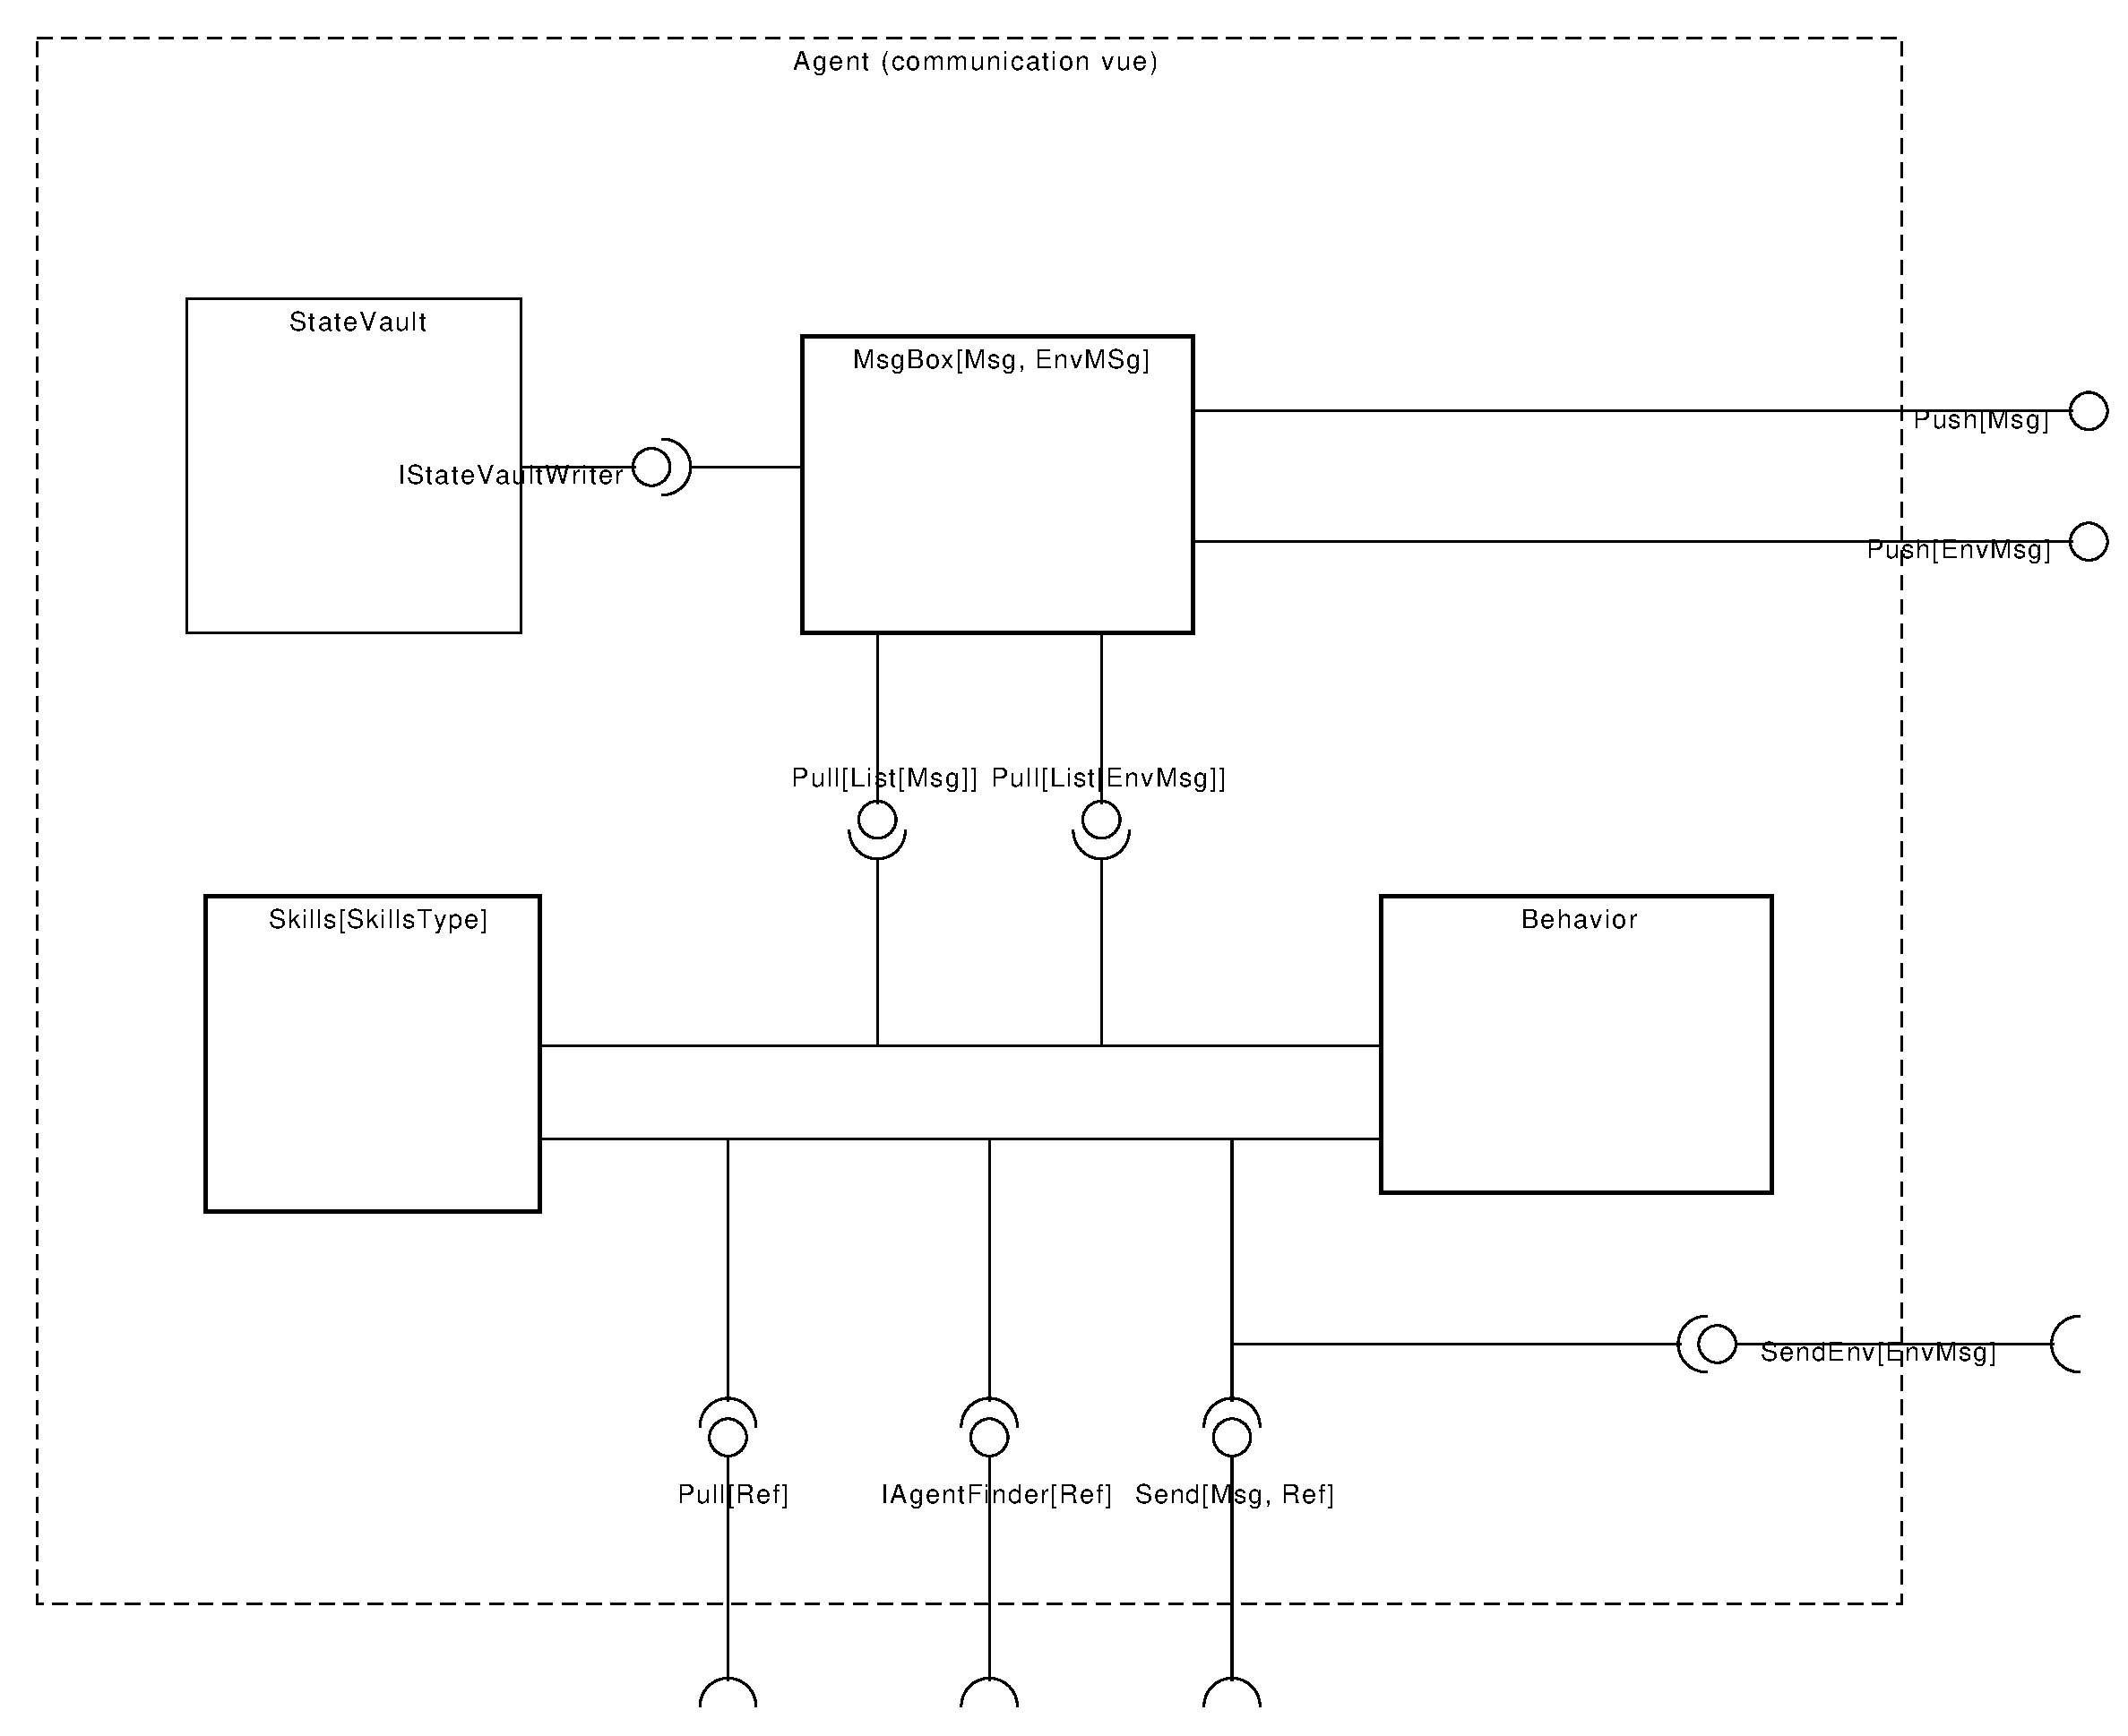
\includegraphics[width=0.6\paperwidth]{ID4CS_Speadl_comm}
\caption{Agent Architecture - Communication view.}
\label{Arch-comm}
\end{figure}

This view contains the new component \emph{Message Box}, which contains the messages sent to the agent. The \emph{Message Box} stores the messages into the \emph{State Vault} and provides a direct access to the \emph{Skills} and {Behavior} components.

This figure presents several ports which need to be provided from the environment to the agent. The environment must give an unique \emph{Reference} to the agent, which will be used by the others agent to communicate with it. The environment must also provides some ports to communicate with the others agents and outside of the system.
[[PARLER DE L'AGENT FINDER ??]]

\subsection{Monitoring}

The \emph{monitoring} view (\figurename{} \ref{Arch-monitor}) presents the components related to the monitoring of the agent. 

The new component introduced in this view is the \emph{Monitor}. The \emph{Monitor} provides to the environment to ports. The first port is used for external monitoring interfaces to subscribe to be informed of changes in the state of the agent. The second is used to provide informations concerning changes of a specific part of the agent. Thus, an external monitoring interface can subscribe to be notified when the state of the agent changed using the first port, and then use the second port to access to the specific informations it want to monitor.

In order to provide its capabilities, the monitor agent need to be informed by the \emph{Behavior} component before and after each step, to read and compare the monitored informations into the \emph{State Vault}.

\begin{figure}
\centering
\includegraphics[width=0.6\paperwidth]{ID4CS_Speadl_monitoring}
\caption{Agent Architecture - Monitoring view.}
\label{Arch-monitor}
\end{figure}

\section{MAS Architecture}

\section{Integration into the prototype}

[[OSGI and EMF]]

This implementation of the MAS was part of a collective development effort to provide a functional prototype. The goal of this prototype is to be a proof-of-concept tool of the possibilities offered by agent-based continuous optimization.

The development of the prototype was carried mainly by three partners[[cite them?]], each in charge of a different aspect.

The prototype can be divided in three parts: The Graphical User Interface (GUI), the core module (CORE) and the Multi-Agent Système (MAS). The CORE provides a common representation of the manipulated data and is in charge of maintaining consistency between the GUI and the MAS.

These three modules communicate using the OSGi framework\footnote{\url{http://www.osgi.org}}.

\subsection{MAS}

We already presented the implementation of the MAS in the previous parts. The only additional work was to encapsulate the implementation into an OSGi [[service]].

\subsection{CORE}

The CORE module is responsible of maintaining consistency of the manipulated data. It serves as a middle-man between the MAS and the GUI.

[[Insert full Data Model and comment]]

\subsection{GUI}

The GUI was build using the [[Eclipse Framework]].




\chapter{Collective Problem Solving Patterns}\label{CPSP}

[[Explain how ADELFE was insufficient to bridge the gap between Abstract spec and implementation => contribution to problem solving AMAS development]]
We have seen in the previous chapter how the ADELFE methodology was used for the design of AMAS, from the general requirement to the implementation of the agents. However a current limitation of ADELFE (shared with most of the existing comparable methods) comes from the fact that it is a general method, which aims to be applicable for design MAS intended for diverse application fields (problem solving, simulation, \emph{etc.}). This desire to be usable in a large spectrum of applications has the drawback that the recommendations and guidelines of ADELFE are of an bastract nature. This make the task of actually designing an AMAS for a precise application difficult for non agent expert, even when the application domain is narrower than, for example, general continuous optimization.\\
This limitation has already been observed in previous works, and has given birth to an ongoing effort to provide a modular toolkit named \emph{AMAS for Optimization (AMAS4Opt}, with the goal to supplement ADELFE and assist AMAS designers when designing MAS for problem solving. In the same way that some contributions have already been proposed in the context of continuous optimization (see \cite{Ka2011.6}), we will now see how we can propose to enrich the toolkit in the context of continous optimization.

In this chapter, we take a step back from the MAS we described in the preceding parts and see how our contribution can be made more general, not only to the benefit of the scientific community, but also for engineers by enriching the AMAS4Opt. Numerical optimization was a mostly unexplored application domain in regard to multi-agents based algorithms. By taking the (somewhat ambitious) task to propose a MAS which would be applicable for this domain in its entirety, some of the patterns identified and some of the mechanisms we proposed can be used in a more general context than our system.

As numerical optimization is in itself an abstract mathematical field, we too had to abstract ourselves from concrete applications. We did not have the possibility to reduce the set of possible configurations and thus we had the occasion to encounter a variety of problems which have been mostly ignored before. Indeed, the graph representations of numerical optimization problems are quite diverse, and can present some topological properties not present in existing MAS formalisms. [[DCOP for example (presented in [[REF]]), ]]

In the description of our system, we presented a set of NCS [[use acronym ?]], and the specifics mechanisms we introduced to handle them. We believe that these NCS are only the instantiation of more general problematic configuration, which we dub \emph{Collective Problem Solving Patterns} (CPSP). The patterns are not restricted to numerical optimization, they can potentially be encountered in all sorts of application domains.

Architecture and software development has greatly benefited from the identification of common design pattern. In the same regard, we believe that the identification of these problem patterns as such, as well as of solution proposals to handle them, could lead to a great improvement for the design of agent-based systems for problem solving as a whole.

Consequently, we will present in this part how the NCS we identified during the design of our system can be abstracted in the broader form of CPSP.


\section{Introduction - Collective Problem Solving Patterns are not Design Patterns}

[[EXPLAIN THE DIFFERENCE WITH EXISTING AGENT PATTERNS]]

Before describing the CPSP in themselves, we must explain how these patterns differ from the existing design patterns for MAS.

There is already an existing (if limited) corpus of design patterns for MAS. These patterns have usually in scope either the design of the organizational structure of system or the design of the behavior architecture of the agents. These patterns concerns the \emph{design} of the system regarding the target application domain. These patterns are relevant in the design of the \emph{organization of the system}, according to the application domain.
What we propose here is a different sort of patterns, which concerns the \emph{behavior of the agent}, according to an existing organization. Design Patterns concern the structural aspects of the system, while Problem Solving Patterns concerns its functional aspects.

In this regard, CPSP are less generic than Design Patterns. Indeed the latter can be applied to the whole range of MAS, while the former only concerns MAS designed for problem solving (excluding, for example, MAS for simulation).

These two kinds of patterns should be seen as complementary. First the designer could use design pattern to design the structure of the MAS according to the needs of the application domain. Then he could use CPSP to identify and solve specific problems resulting from such modeling.

As we want a description of our patterns which is domain-free, we cannot re-use the modeling we introduced in \ref{modeling}. The NDMO formalism is indeed bound to the domain of numerical optimization. Consequently, we will now introduce a higher-level formalism, which concentrates on the relations between the agents of the system. to keep this formalism short and simple, we will make some assumptions about the functioning of the system.

We will consider systems composed of autonomous agents and resources. An agent may needs for one or more resources to be in a specific state to accomplish its local goal. We will suppose that a resource is controlled by one agent and one agent only. We believe that this simplifying assumption does not impede on the generality of the formalism (for example a system where two agents share the control of a resource can be viewed as equivalent to a system where both agents send requests to a third one solely in charge of it).

[[are these assumptions correct ??]]
To formalize the resources, we will consider each resource as a variable which can be assigned a number from a set representing its different possibles states. As most multi-agent systems manipulate numeric values, or data which can be represented by numeric values, this representation can be translated quite straightforwardly to most specifics cases.
The states represented by these numbers can be inherent to the resource, such as a color assigned to it in the graph coloring problem, or indicate the fact that the usage of the resource is attributed to a specific agent as in auction-based systems.

We will suppose that agents interact among themselves by message passing.

\section{Description of a Problem Solving Pattern}

\subsection{Agent Roles}

Concerning the patterns we present in this article, we identified three different types of agent \emph{roles}: Provider, Solicitor and Transformer.

The \emph{Provider} role represents the fact that the agent is in charge of a given resource, which can be of use to others agents in the system. The agent is responsible of choosing the state of the resource or giving access to it based on solicitations of others.

The \emph{Solicitor} role represents the fact that the agent requires some resource(s) which it does not control to be in a specific state, in order to accomplish its goal. Consequently, the agent needs to solicit the agent(s) controlling the relevant resource(s).

The \emph{Transformer} role is a combination of the Provider and Solicitor roles. The transformer agent controls a resource but the state of the resource is dependent of some other resources not controlled by the agent. While this role can be represented by assigning both Provider and Solicitor roles to the agent, we found it common enough to be worth of a specific representation. As we will see, transformer agents sometimes play a specific role in the CPSP, as they can be a source of delay or obfuscation of information.

On \figurename{} \ref{cpsp_class_diag} is shown the very simple class diagram representing the relationships between these three roles.

\begin{figure}
\centering
\includegraphics[width=0.5\textwidth]{cpsp_class_diag-crop}
\caption{class diagram of the Provider-Solicitor modeling}
\label{cpsp_class_diag}
\end{figure}

It is important to understand that an agent is not limited to one role only. For a given system an agent can, depending on the context, assume any combination of these roles. Thus an agent can both solicit others agents regarding a resource, while providing a controlled resource to others agents.
In this regard, an agent can even be a producer and solicitor of the same resource. For example the agent is in charge of a specific resource, but also benefit from it. In this case the agent can possibly be in conflict with others agents regarding the state of the resource, and decide (as a producer) to go against its own interest (as a solicitor) in order to help another agent deemed more important.
Obviously, in most implementations, the different roles of the agent would not be as much segregated, and the agent would not strictly communicate with itself using message-passing. This distinction should not be a problem in practice (this kind of configuration can however trigger others CPSP, see for example \ref{NCS_async}).

\subsection{Problem Pattern}

[[Name, Description, Minimal Form, Alternates forms, Symptoms, Solution(s)]]

\subsection{Solution}

\section{Identified Collective Problem Solving Patterns}

In this section, we present the CPSP we identified from the NCS we encountered during the design of our MAS.

\subsection{Conflicting Requests and Criticality}

\subsection{Cooperative Trajectories}

\subsection{Cycle Solving}

\subsection{Hidden Dependencies}

\subsection{Asynchronous Requests}

\section{Conclusion on Collective Problem Solving Patterns}

[[TODO: add some text]]

We identified these patterns from the the NCS of our system. In reverse, the NCS used in the design of AMAS seems perfectly adequate to instantiate known CPSP. Indeed, subsumption-based behavior architectures are very appropriate to model this kind of \enquote{exception}-like situations. Should this kind of patterns identification and reuse becomes more wildly used, one could expect this way of modeling agent behavior to becomes quite popular.

\part{Experiments and Validation}

In this section we present three test cases, Alexandrov Problem, Turbofan Problem and Viennet1, on which our system has been applied, and the experimental results we obtained. In each test cases, the MAS consistently converges towards the best (or one of the best) solution.

\begin{figure}
\centering
	\subfloat[mathematical formulation.]{\begin{minipage}{0.4\textwidth}%
		$\begin{array}{c}
			a_1 = (l_1 - a_2)/2 \\
			a_2 = (l_2 - a_1)/2 \\
			min \; \frac{1}{2}(a_1^2 + 10a_2^2 + 5(s-3)^2) \\
			subject \; to \\
			s + l_1 \leq 1 \\
			-s + l_2 \leq -2
		\end{array}$
		\label{alexandrov:math}
	\end{minipage}}\hfill%for spacing
	\subfloat[corresponding agent graph.]{\begin{minipage}{0.5\textwidth}%
		\centering
		\includegraphics[width=\textwidth]{testcases-Alexandrov}%screen_Alexandrov}%}
		\label{alexandrov:graph}
	\end{minipage}}
	\caption{Alexandrov problem}
	\label{alexandrov}
	\vspace{-20pt}
\end{figure}

\subsection{Alexandrov Problem}

\begin{figure}[t]
\centering

  \subfloat{\begin{minipage}{0.4\textwidth}%
		\centering
		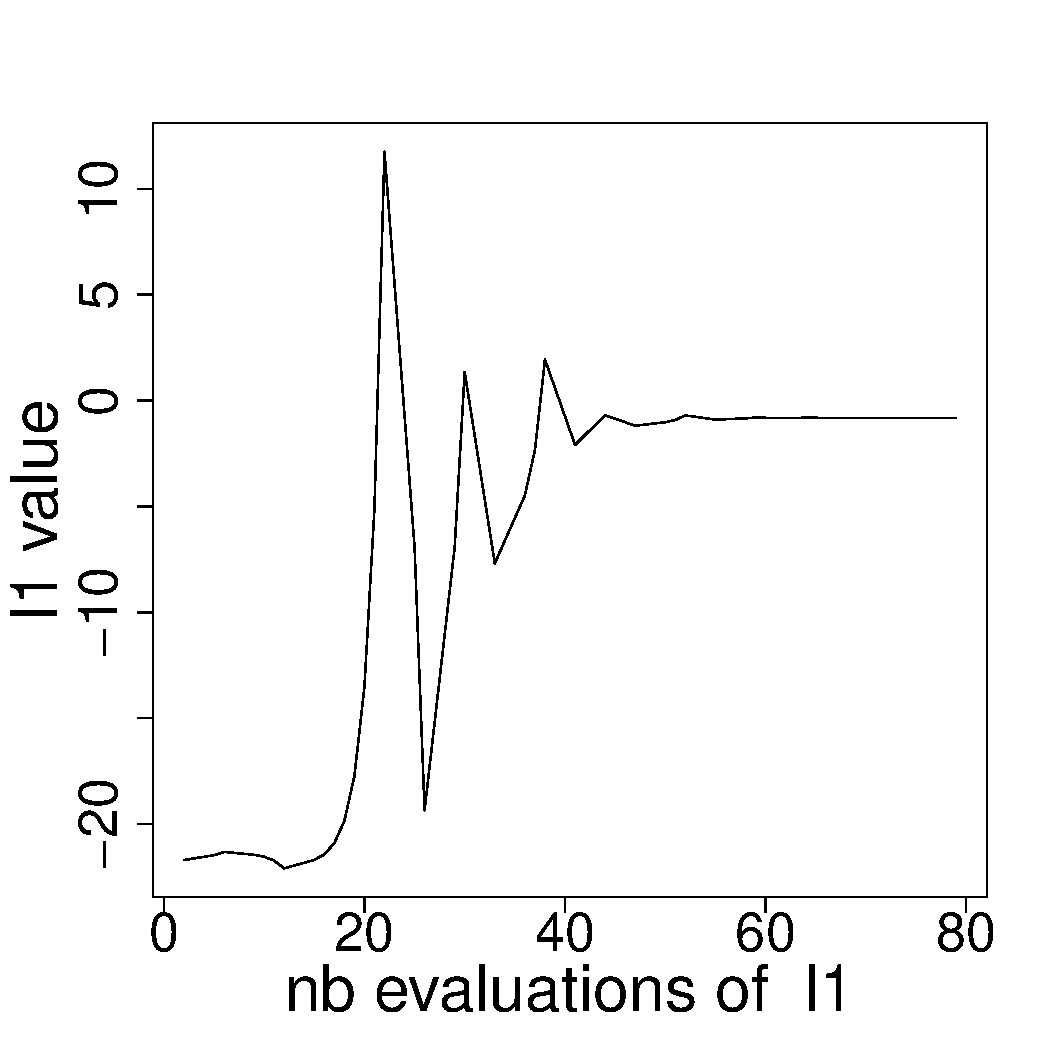
\includegraphics[width=\textwidth]{./R_figs/generated/l1_one_run}
		\vspace{-20pt}
		\label{alexandrov_res_one:l1}
	\end{minipage}}%
	\subfloat{\begin{minipage}{0.4\textwidth}%
		\centering
		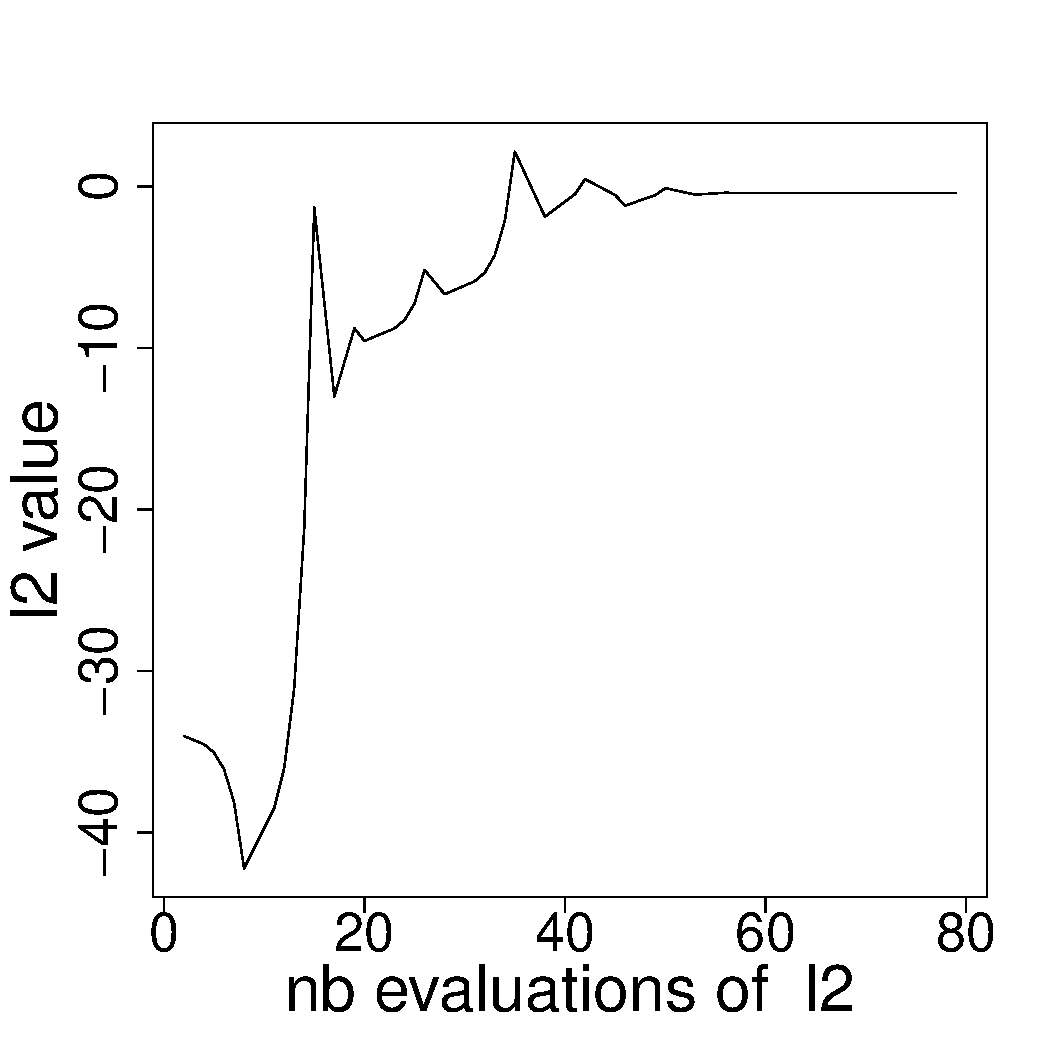
\includegraphics[width=\textwidth]{./R_figs/generated/l2_one_run}
		\vspace{-20pt}
		\label{alexandrov_res_one:l2}
	\end{minipage}}
	\vspace{-20pt}
	\\
	\subfloat{\begin{minipage}{0.4\textwidth}%
		\centering
		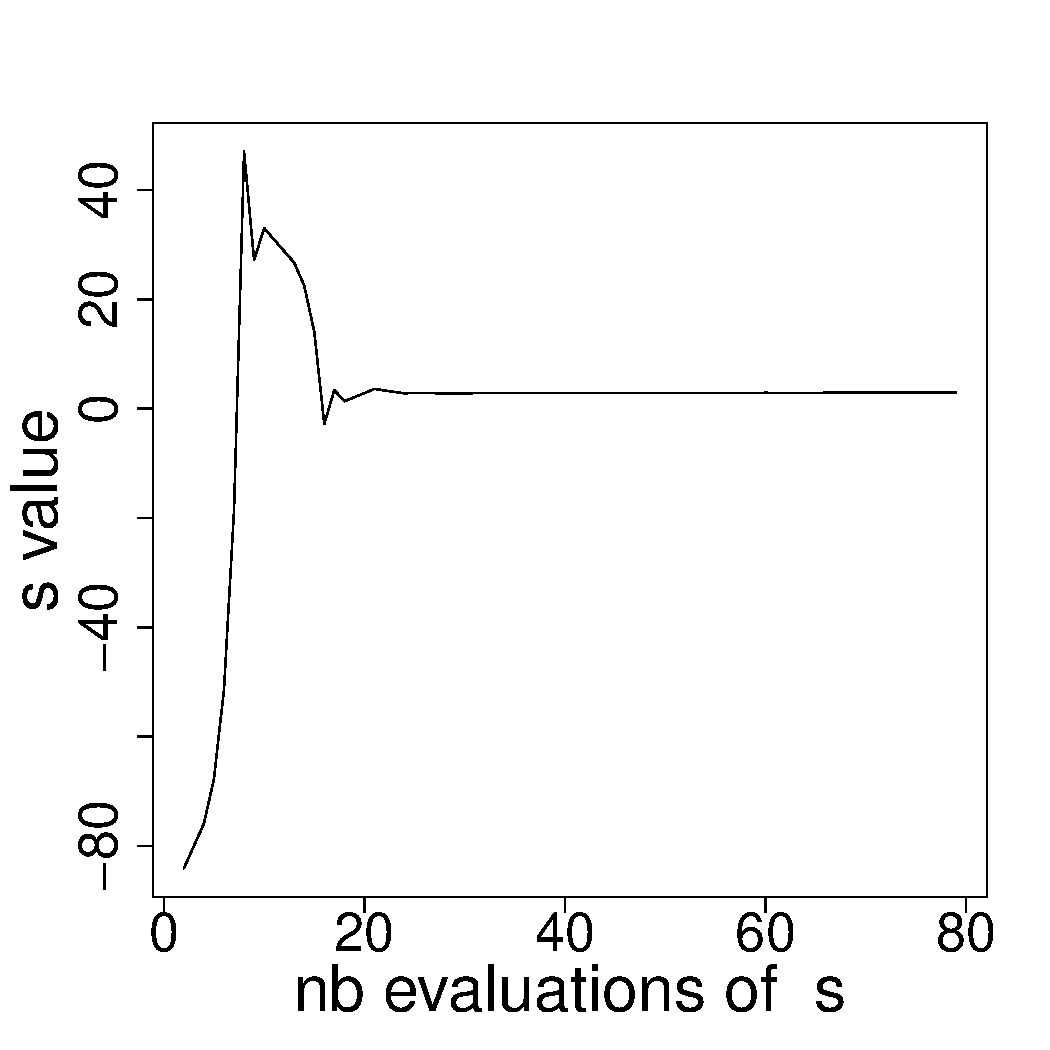
\includegraphics[width=\textwidth]{./R_figs/generated/s_one_run}
		\vspace{-20pt}
		\label{alexandrov_res_one:s}
	\end{minipage}}%
	\subfloat{\begin{minipage}{0.4\textwidth}%
		\centering
		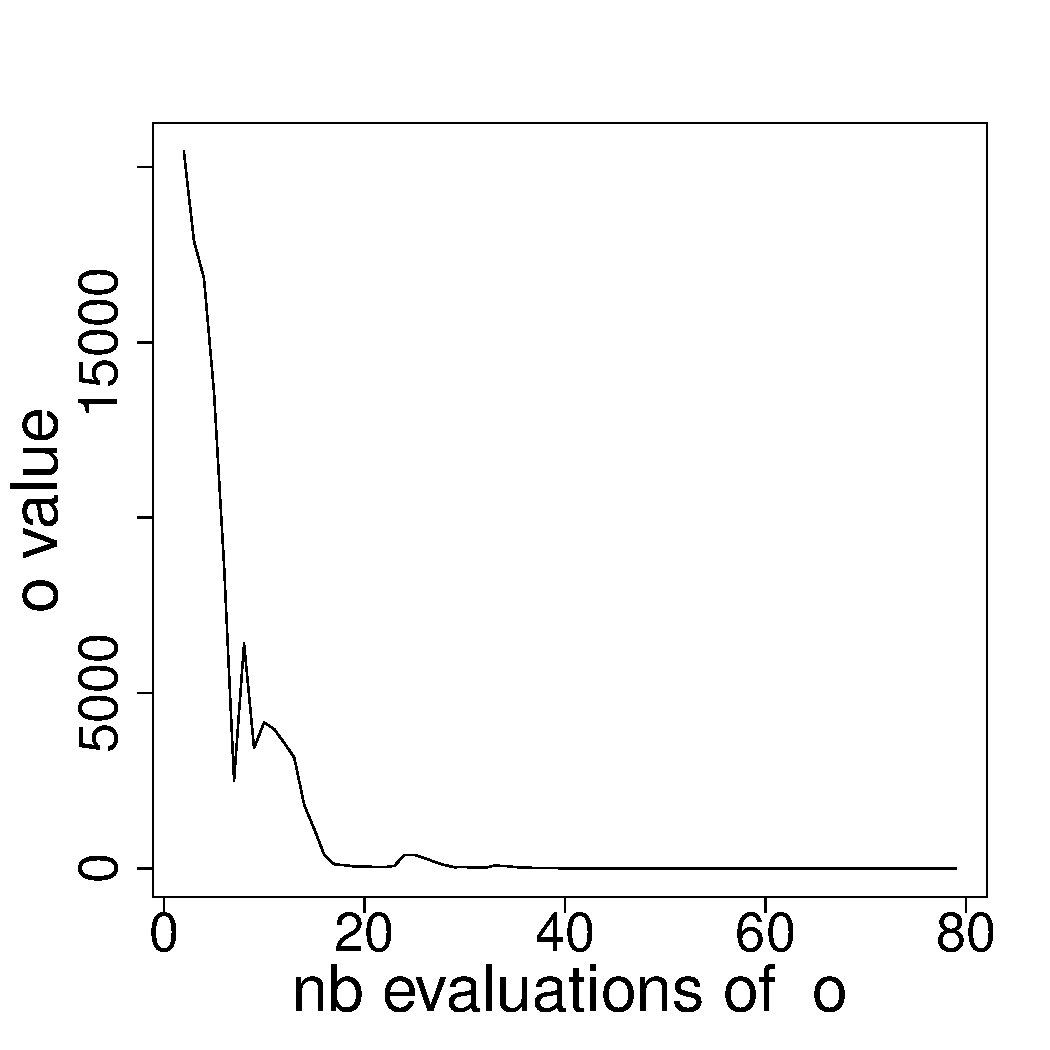
\includegraphics[width=\textwidth]{./R_figs/generated/o_one_run}
		\vspace{-20pt}
		\label{alexandrov_res_one:o}
	\end{minipage}}%
	
	\caption{Alexandrov agents behavior}
	\label{alexandrov_res_one}

\end{figure}

\begin{wrapfigure}{R}{0.4\textwidth}
	\vspace{-50pt}
    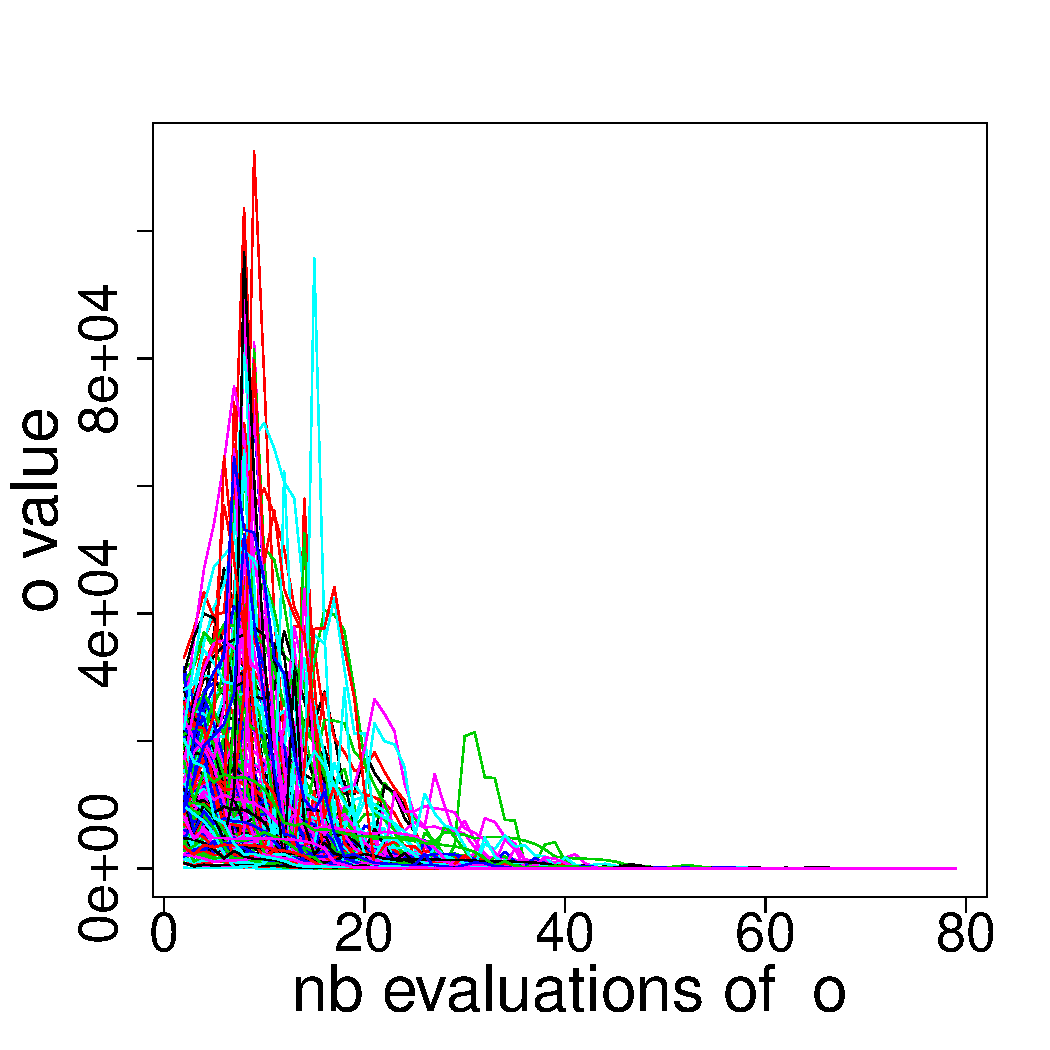
\includegraphics[width=0.4\textwidth]{./R_figs/generated/o}
	\caption{Convergence of the Alexandrov objective for 100 random starting points}
	\label{alexandrov_res}
	\vspace{-25pt}
\end{wrapfigure}

Our first test case is inspired from an academic example taken in literature by Alexandrov and al\cite{alexandrov2002analytical}. This simple example presents some of the commons characteristics of MDO problems, such as interdependent disciplines and multiple criteria. In the original article, the example was used to illustrate some properties of Collaborative Optimization, which we presented earlier, in terms of reformulation. While the paper only gave the structure of the problem, we adapted it with meaningful values and equations.
The mathematical formulation of the problem and the corresponding agent graph can be seen in \figurename \ref{alexandrov}. Interestingly, the NDMO representation is quite similar to the one adopted by the original authors of the problem.

On \figurename \ref{alexandrov_res_one}, the behavior of the \emph{design variables} agents l1, l2 and s, as well the evolution of the objective, can be observed on one instance of the problem with random starting points. On \figurename \ref{alexandrov_res}, we show the evolution of the objective over 100 iterations with  starting points  for each \emph{design variable} randomly drawn over the interval [-100; 100]. We can see how the system converges towards the same optimum despite the wildly different initial conditions.

\subsubsection*{Adaptation to perturbations}
 
On \figurename \ref{alexandrov_res_pert}, we can observe the reaction of the multi-agent system to a perturbation. During the solving of the previous problem, we changed the threshold of the constraint $s + l_1 \leq 1$ to $s + l_1 \leq -4$ (the change is indicated by a dotted line on the charts). The system dynamically adapts to the constraint changed and converges towards a new solution which satisfies the updated constraint.


\begin{figure}[h]
\centering

  \subfloat{\begin{minipage}{0.4\textwidth}%
		\centering
		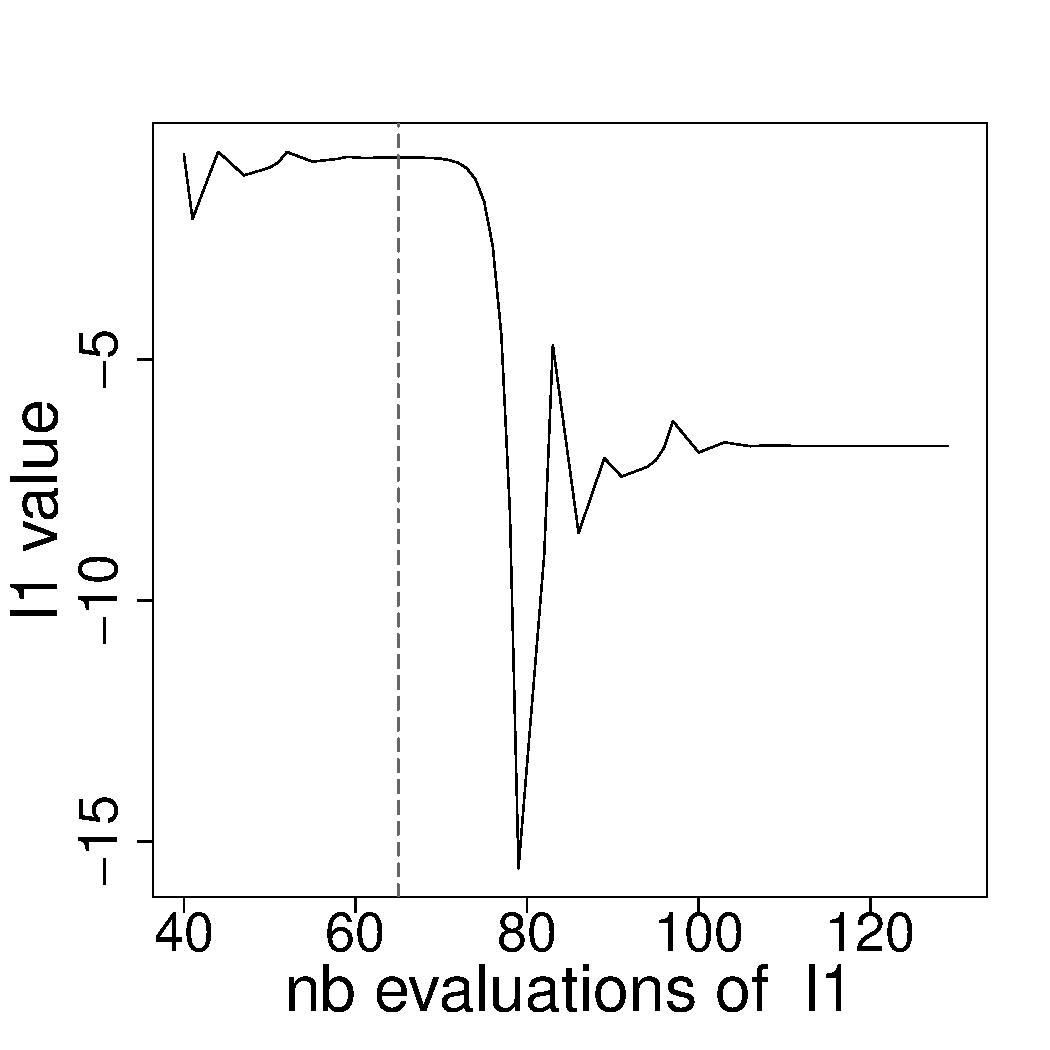
\includegraphics[width=\textwidth]{./R_figs/generated/l1_pertubated}
		\vspace{-20pt}
		\label{alexandrov_res_pert:l1}
	\end{minipage}}%
	\subfloat{\begin{minipage}{0.4\textwidth}%
		\centering
		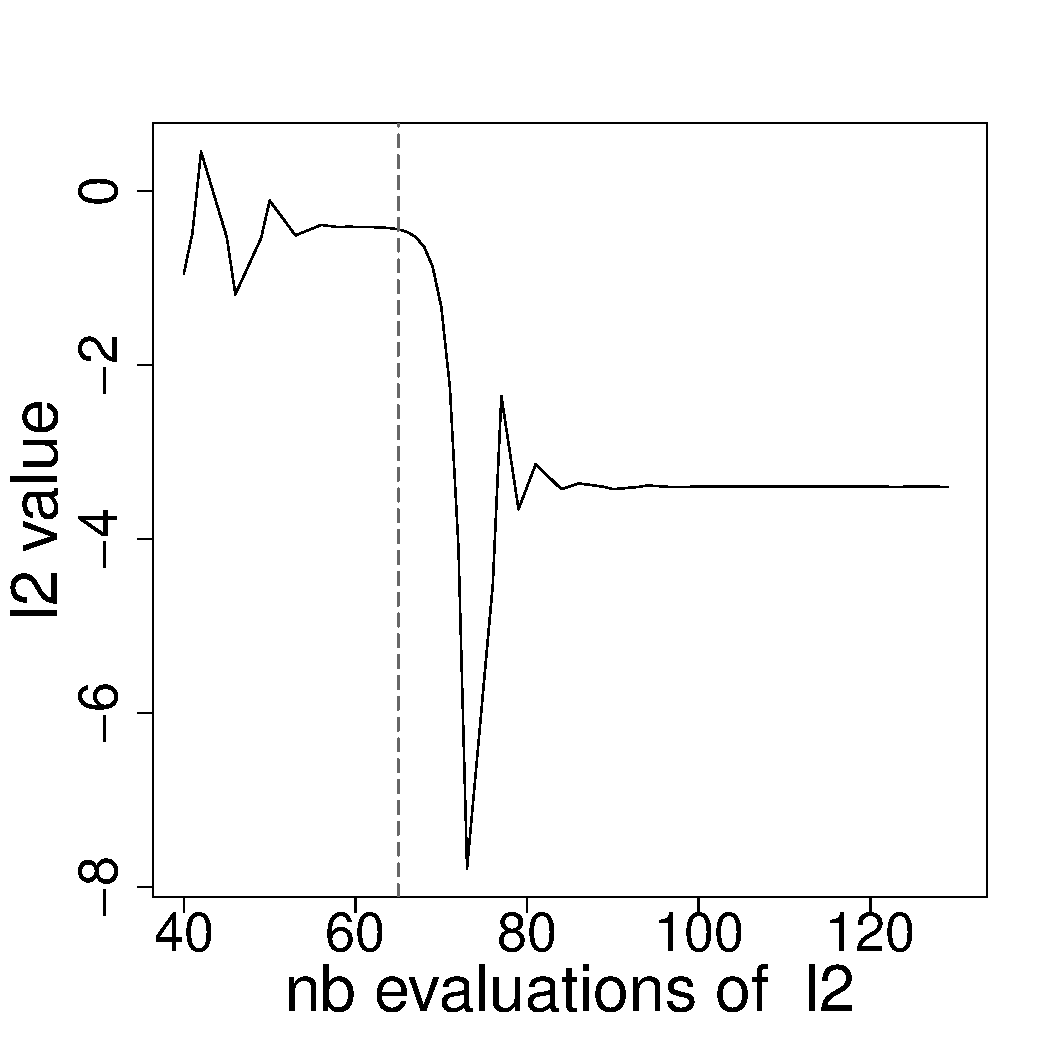
\includegraphics[width=\textwidth]{./R_figs/generated/l2_pertubated}
		\vspace{-20pt}
		\label{alexandrov_res_pert:l2}
	\end{minipage}}
	\vspace{-20pt}
	\\
	\subfloat{\begin{minipage}{0.4\textwidth}%
		\centering
		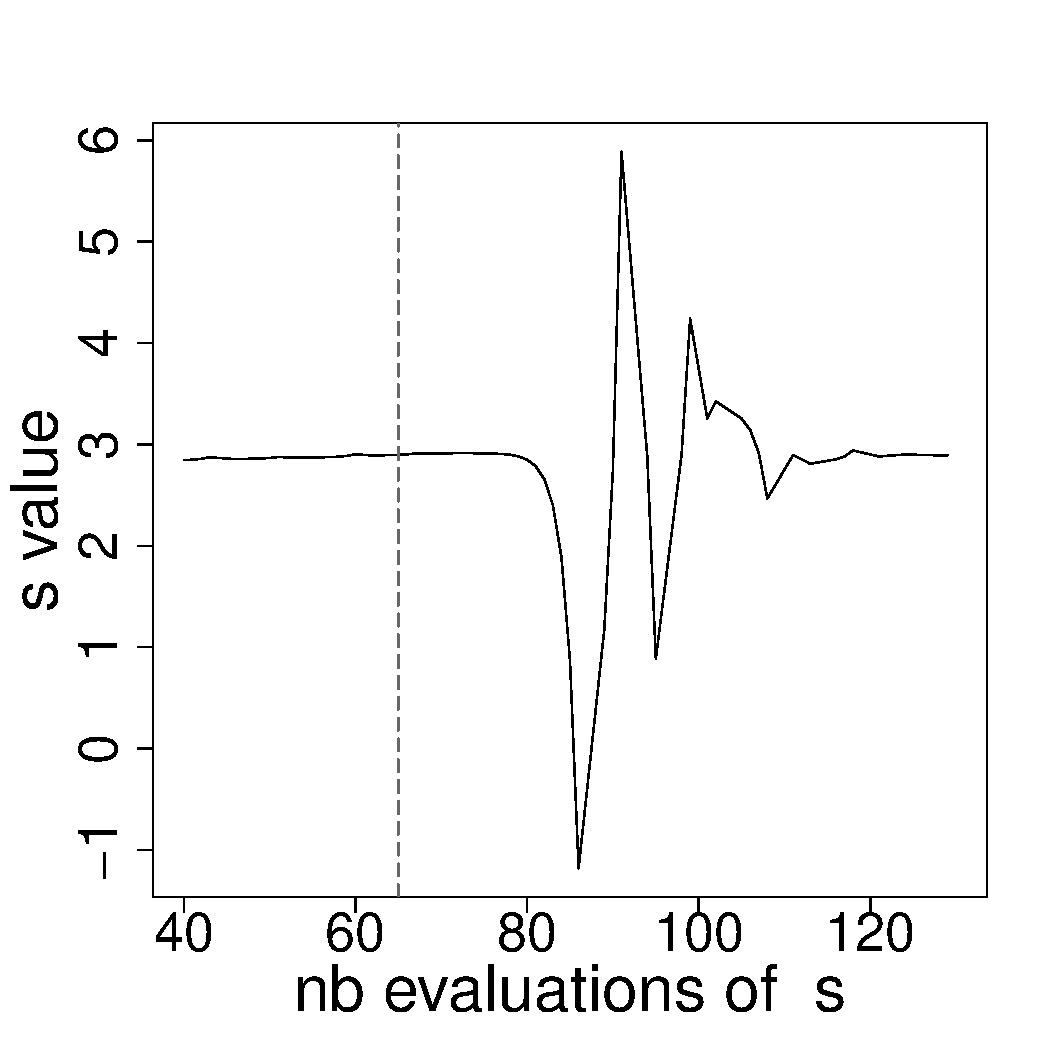
\includegraphics[width=\textwidth]{./R_figs/generated/s_pertubated}
		\vspace{-20pt}
		\label{alexandrov_res_pert:s}
	\end{minipage}}%
	\subfloat{\begin{minipage}{0.4\textwidth}%
		\centering
		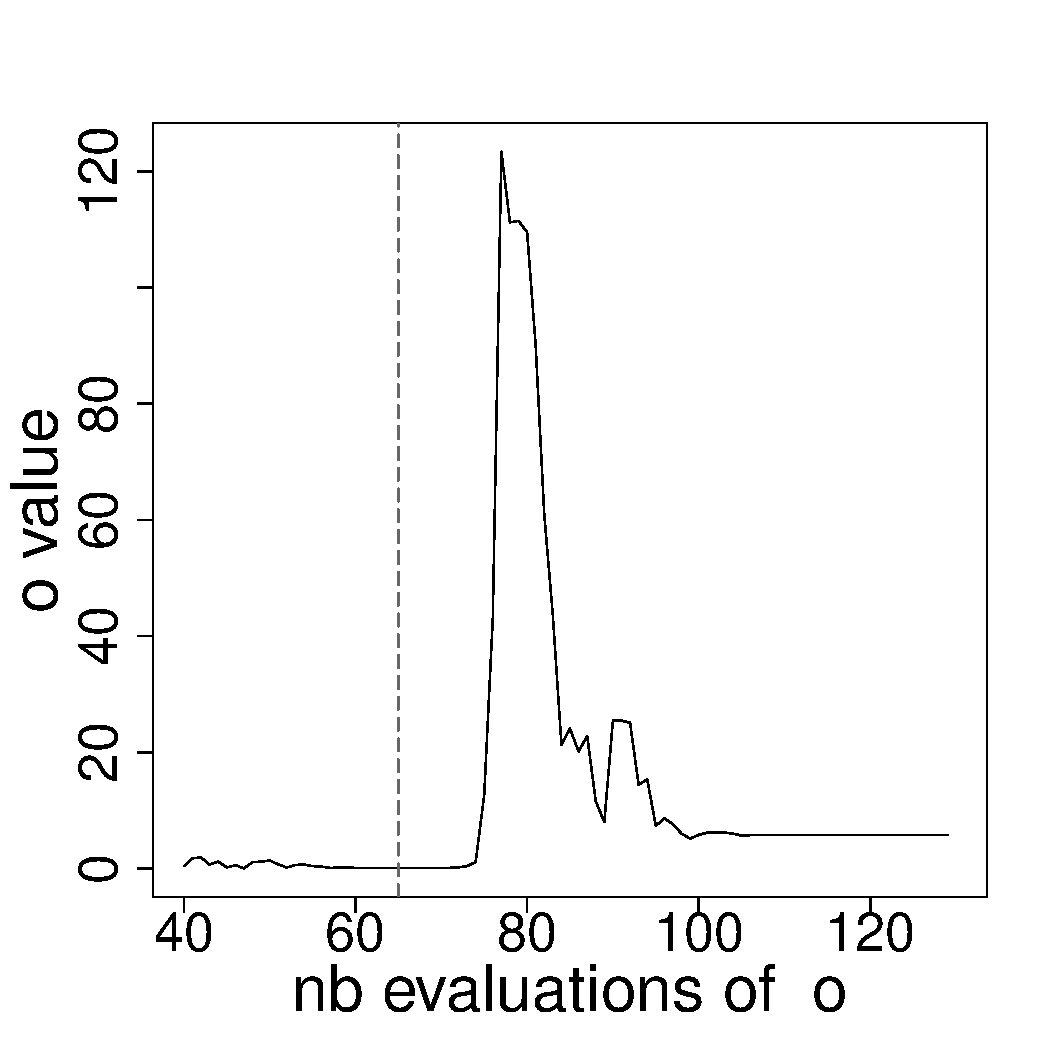
\includegraphics[width=\textwidth]{./R_figs/generated/o_pertubated}
		\vspace{-20pt}
		\label{alexandrov_res_pert:o}
	\end{minipage}}%
	
	\caption{Alexandrov agents behavior with perturbation (constraint change at dotted line)}
	\label{alexandrov_res_pert}

\end{figure}


\subsection{Other Experiments}

We now briefly present results we obtained on two others test cases, the Turbofan problem and Viennet1. For each case, the system was executed 100 times with random starting points for each \emph{design variable}.

\subsubsection{Turbofan Problem}

The turbofan problem we introduced in \figurename \ref{turbofan} is a based on a real-world optimization problem, albeit simplified for demonstration purpose, concerning the conception of a turbofan engine.

As stated before, the problem concerns two \emph{design variables} $pi\_c$ and $bpr$. $pi\_c$ is defined inside the interval [20-40] and $bpr$ inside [2-10]. The model produces three variables $Tdm0$, $s$ and $fr$.
The problem has two objectives, maximizing  $Tdm0$ and minimizing $s$, under the constraint \(s \leq 155\) and \(fr \geq 4\).
The main interest and difficulty of this problem is the existence of two contradictory objectives.
As we can see on \figurename \ref{snecma_res}, the system consistently converges toward the same optimal solution.

\begin{figure}[h]
	\subfloat{\begin{minipage}{0.49\textwidth}%
		\centering
		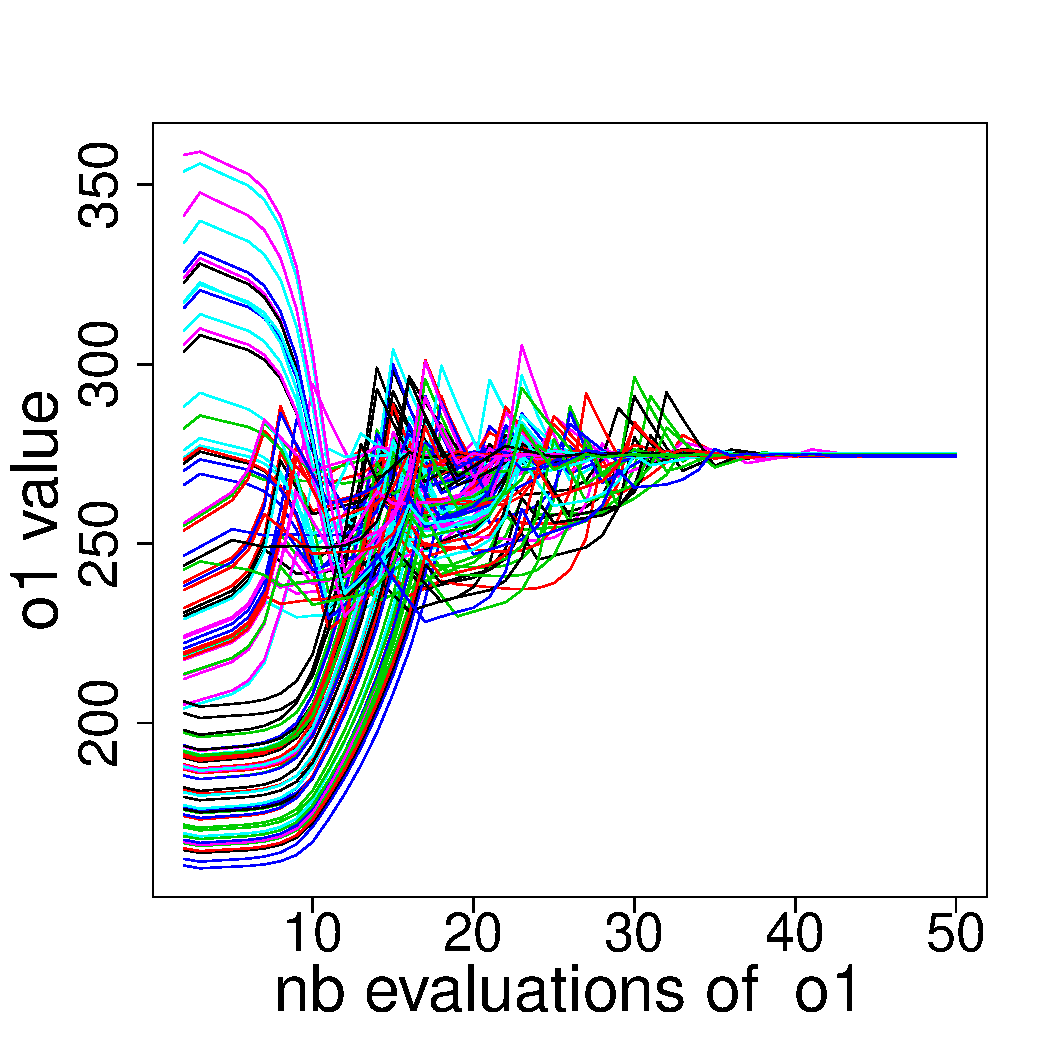
\includegraphics[width = \textwidth]{./R_figs/generated/o1}	
	\end{minipage}}%
	\hfill%for spacing
	\subfloat{\begin{minipage}{0.49\textwidth}%
		\centering
		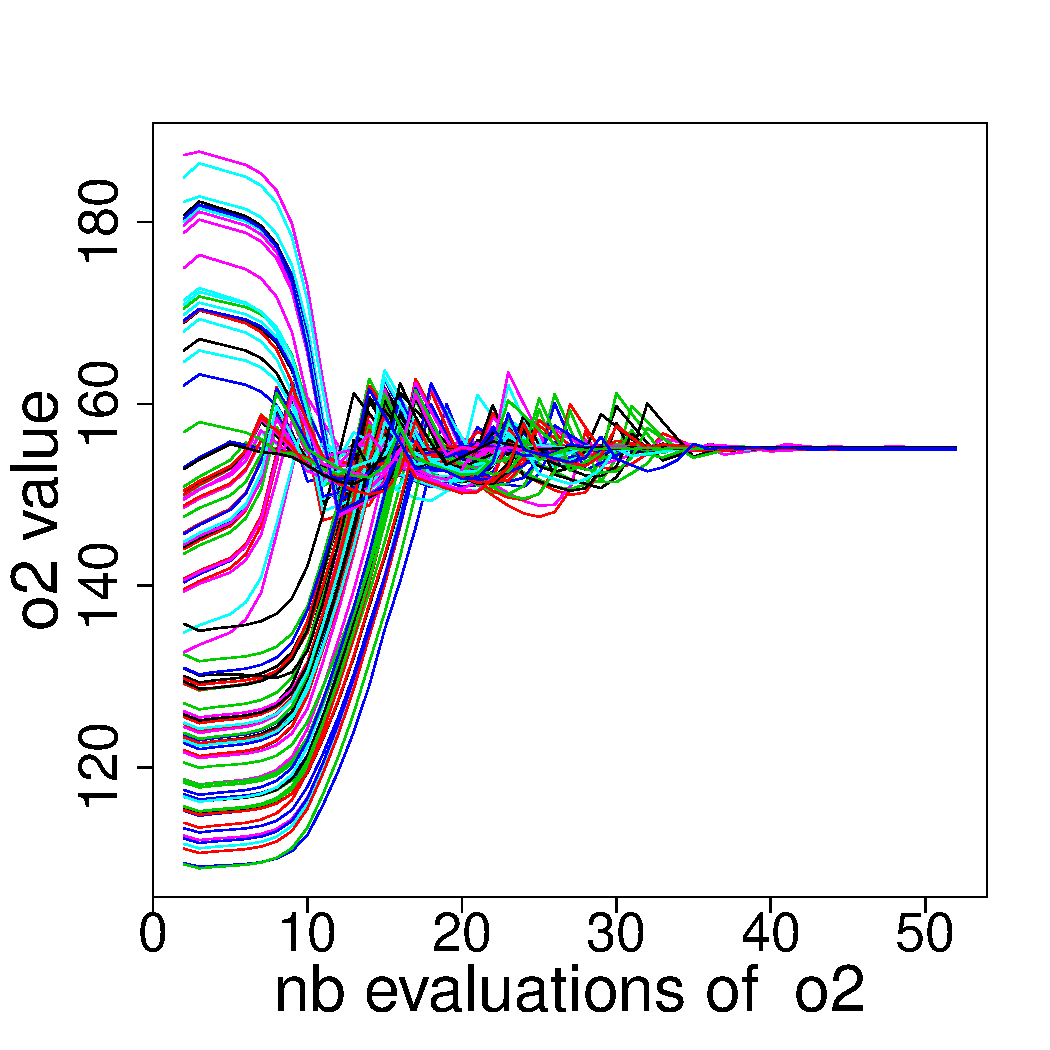
\includegraphics[width = \textwidth]{./R_figs/generated/o2}	
	\end{minipage}}%
	\caption{Convergence of the Turbofan objectives for 100 random starting points}
	\label{snecma_res}
\end{figure}

\subsubsection{Viennet1}

The Viennet1 test case is part of a series of problems proposed in \cite{viennet1996multicriteria} to evaluate multi-criteria optimization techniques. This problem involves three objectives. Its analytical formulation is:


$$\text{Minimize } o1 = x^2 + (y-1)^2 \text{, } o2 = x^2 + (y+1)^2 \text{ and } o3 = (x-1)^2 + y^2 +2\\$$
$$\text{where } x, y \in  [-4;4]
$$

\figurename \ref{viennet_res} illustrates the convergence of the system towards a valid solution.


\begin{figure}[h]

	\subfloat{\begin{minipage}{0.33\textwidth}%
		\centering
		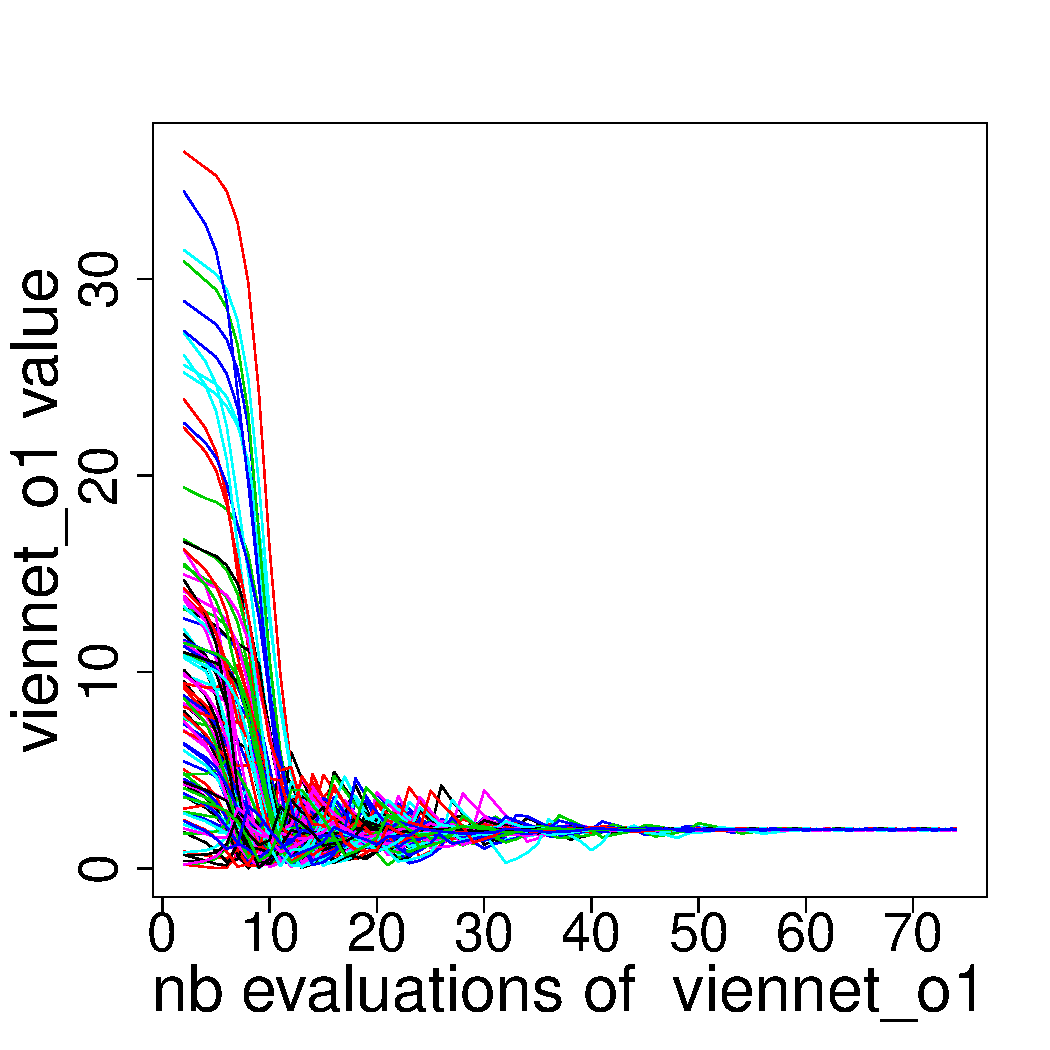
\includegraphics[width = \textwidth]{./R_figs/generated/viennet_o1}	
	\end{minipage}}%
	\hfill%for spacing
	\subfloat{\begin{minipage}{0.33\textwidth}%
		\centering
		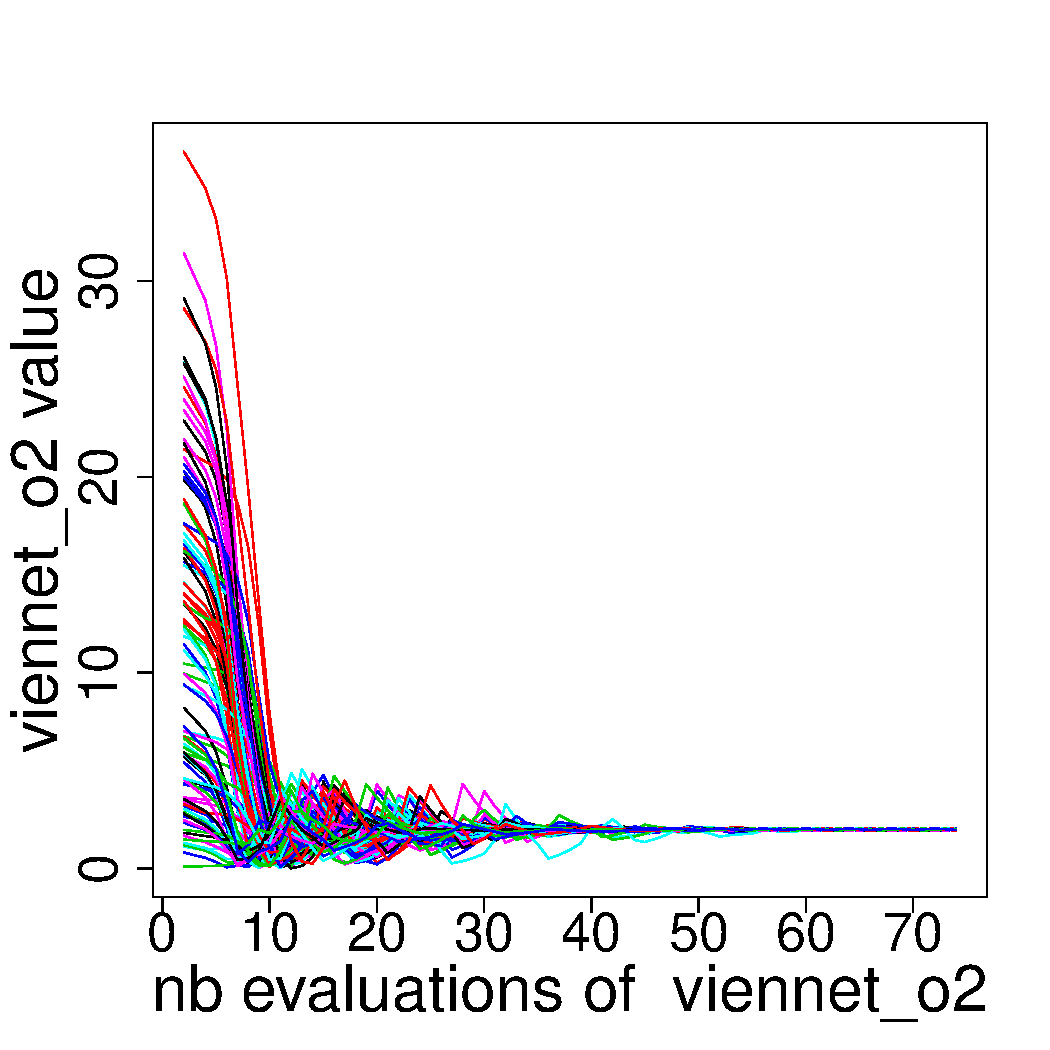
\includegraphics[width = \textwidth]{./R_figs/generated/viennet_o2}	
	\end{minipage}}%
	\hfill%for spacing
	\subfloat{\begin{minipage}{0.33\textwidth}%
		\centering
		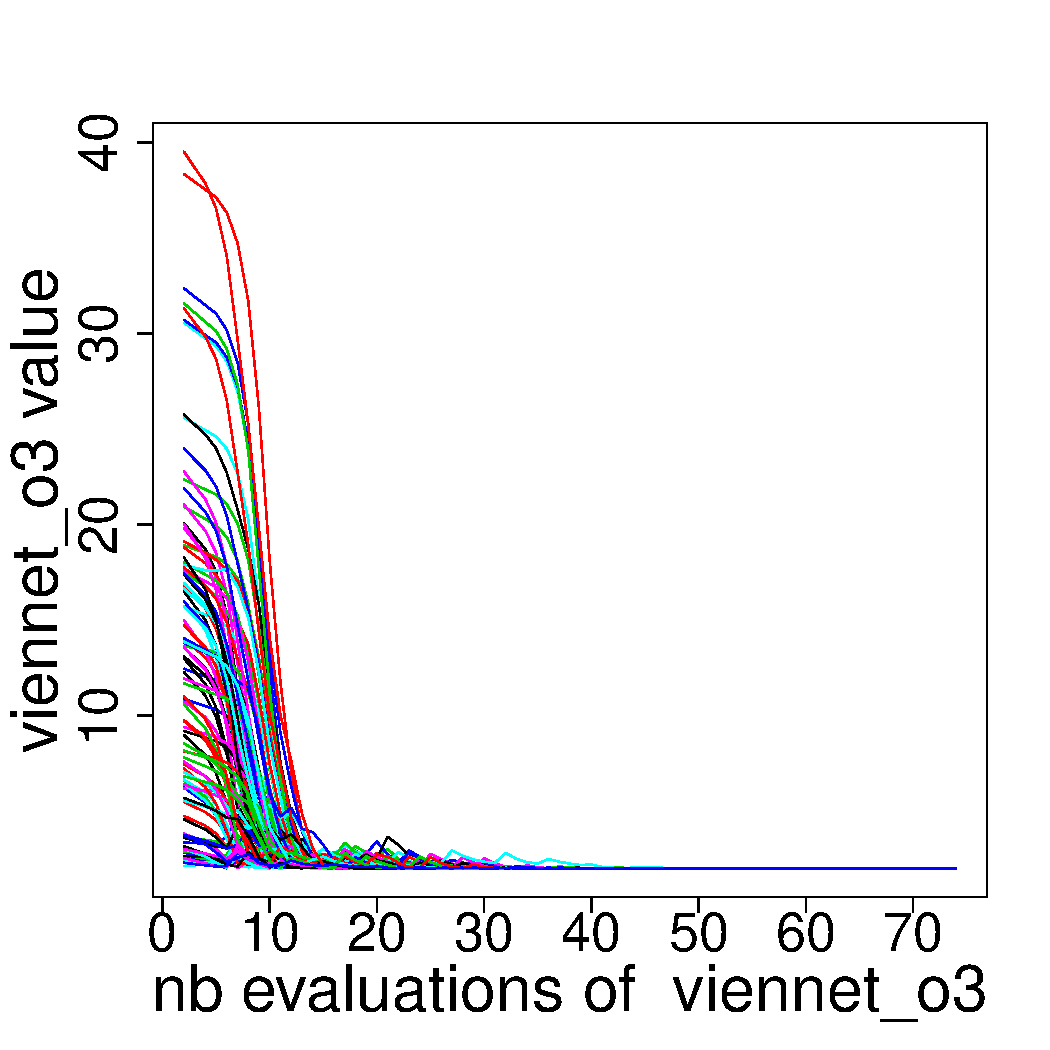
\includegraphics[width = \textwidth]{./R_figs/generated/viennet_o3}	
	\end{minipage}}%
	\caption{Convergence of Viennet1 objectives for 100 random starting points}
	\label{viennet_res}
\end{figure}

\subsubsection{Rosenbrock's valley}

Rosenbrock's valley is non-convex function commonly used to test convergence performances. The results presented here are for the two-dimensional version of the problem with a definition domain of [-5; 5] for each \emph{design variable}.
The analytical formulation of this problem (for two dimensions) is 
$$\text{Minimize } f(x,y) = (1-x)^2 + 100(y - x^2)^2$$

\begin{wrapfigure}{R}{0.5\textwidth}
    \vspace{-50pt}
    \includegraphics[width = 0.5\textwidth]{./R_figs/generated/minimizer}	
    	\vspace{-30pt}
	\caption{Convergence of Rosenbrock objective for 100 random starting points}
	\vspace{-20pt}
\end{wrapfigure}

%%%%%%%%%%%%%%%%%%%


\Conclusion{Conclusion and Perspectives}

In this thesis we identified a severe limitation of current continuous optimization methods regarding the handling of complex continuation problem. Problems of this category are usually too complex to be solved by classical optimization methods because of multiple factors: the interdependencies of their components, their heavy computational cost, their nonlinearities \emph{etc.} This limitation has been the motivation to propose new specific methods which divide the problem into several disciplines and distribute the optimization process using discipline-level optimizers. However these methods are often difficult to put in practice and cumbersome, not suiting the need of a flexible and iterative process often associated with such problems.

\section*{Thesis Contributions to Continuous Optimization}

This thesis proposes a \textbf{new approach for solving complex continuous problems using an adaptive multi-agent system}. This system, designed following the Adaptive Multi-Agent Systems theory, proposes a decentralized way to automatically distribute the optimization process among the agents, and is able not only to solve large-scale complex problems, but also to adapt to changes made by the user during optimization.\\
The scalability of our approach is made possible by the fact that the agents keep a local view of the system. The system adapts to changes by propagating them from neighbor to neighbor, enabling the \textbf{interactive co-design of the solution}.

This system is built upon a \textbf{general continuous problem modeling we named Natural Domain Modeling for Optimization}, which transform the optimization problem into an entities graph. \textbf{This transformation does not require any simplification, modification or reformulation of the original problem and is fully automatic}.

Following the AMAS theory, we kept the agent perceptions and capabilities at a local level, allowing them to communicate and interact only with their immediate neighbors. Doing so, we are able to handle the problems complexity, as each agent keeps a local point-of-view. The agents are able to use external optimization tools (or can alternatively use local approximation techniques) to solve their local optimization problems. \textbf{This local optimization behavior, along with the message-based global consistency, enables a nominal distributed optimization process}.

We identified several configurations that are susceptible to disturb the good functioning of our system optimization process, corresponding to Non Cooperative Situations (NCS) of the AMAS theory. While these NCS can arise from the interaction of several agents, the agents had to be able to detect and solve them using only local mechanisms. \textbf{For each NCS we proposed local cooperative behaviors for the agents to be able able to cooperatively solve the situation and restore the correct optimization flow}. These cooperative behaviors use specific mechanisms and measures in order to correctly identify the NCS and take the adequate corrective action.

We proved the modularity of our design by showing how our system could be modified to handle additional concerns. To illustrate this, we \textbf{integrated in the agent mechanisms for managing the uncertainties propagation}, effectively allowing the system to realize optimization under uncertainties.

At last, we validated our approach on several test cases. We also integrated our system into a prototype in the context of the ID4CS project funded by the French National Research Agency, prototype currently tested by our industrial parters Airbus and Snecma.

\section*{Thesis Contribution to Multi-Agent Systems}

We already introduced how our identification of specific NCS led to the development of specific agent mechanisms in order for the system to maintain a correct behavior, such as cooperative trajectories, cycle solving \emph{etc.} Based on these NCS and solving mechanisms, we proposed more general Collective Problem Solving Patterns (CPSP). \textbf{These CPSP provide some guidance to the MAS designer regarding some potentially problematic agent configurations which may happen in the system, and propose some solving mechanisms to handle these situations.} We illustrated these CPSP with blueprints summarizing the configuration and mechanisms involved.\\
This work contributes to the ongoing effort of creating general tools for the design of AMAS in the context of problem solving, regrouped under the name AMAS4Opt (Adaptive Multi-Agents Systems for Optimization).

Using the Make Agents Yourself framework, we proposed \textbf{a modular agent architecture adapted to the modeling of hierarchical AMAS agent roles}, based on reusable \enquote{building blocks}. This architecture use a composition of stackable \enquote{skills} components, which allows for an efficient implementation of the handling of the different NCS by the agents.\\
This architecture can be used by the MAS designer as a base to design his own agents, using existing components, and contribute to the effort of providing tools for MAS engineering.

We proposed \textbf{a general graph representation of continuous optimization problems, which can be re-used by MAS designers as a common base to propose other MAS-based approaches for continuous optimization}. Using this common representation, such methods will be easier to compare in terms of solving mechanisms and performances.

\section*{Scientific Perspectives}

\subsection*{Perspectives on MAS for Continuous Optimization}

In regard of continuous optimization, our system could be enhanced with several additional capabilities. Currently, our system concentrates on providing \emph{one} optimal solution. An obvious improvement would be to modify the agents to explore the Pareto front and provide several optimal solutions to the problem. A possible lead would be to modify the objective agents handling of criticality, in order to modulate the weight associated with each objective.

Another possible improvement for designers would be to integrate multi-fidelity models in the system. Multi-fidelity model is a technique to reduce the computational cost of optimization, using several versions of the same model with different computational costs. The low-cost, imprecise models are used at the start of the optimization process, while the high-cost, high-fidelity models are used when the system is starting to converge, in order to improve the precision of the solution. A difficulty of such mechanisms is the maintaining of the consistency between the different levels. This kind of mechanisms could be implemented in our system through the behavior of model agents.

The use of external optimizers could be improved by providing automated optimizer selection mechanisms, in order for the agents to be able to select the most appropriate optimizer, or even change of optimization method during the solving process. Such improvement would possibility require the creation of an optimization ontology in order to characterize the different optimizers.

One could imagine to add self-organizing capabilities to the system, in order to automatically compose the agent graph representing an optimization problem. Such functionality could be used, for example, to provide assistance to the designer during the specification of the optimization problem.\\
With such mechanisms, the user would only have to define a base of elements (variables, models, criteria \emph{etc.}) and the system would be able to automatically assemble the elements into an agent graph, possibly creating (or requesting to the user) new elements as needed. Such functioning would be made possible more easily by the fact that the NDMO formalism does not necessitate any specific formulation to be valid.

\subsection*{Perspectives on the Design of MAS and CPSP}

Concerning the design of MAS, we believe that both researchers and engineers would benefit greatly from the creation of an agent patterns repository. We intend to provide a more detailed and standardized description of the Collective Problem Solving Patterns we identified, with the goal of having a self-sufficient specification document.

An obvious continuation of this work is the identification of new CPSP, either concerning configurations we failed to identify in our application, or with configuration which appear in other application domains. Another possibility concerns the development of alternate handling mechanisms for existing CPSP.

An interesting addition to the CPSP would be to provide an implementation of specialized components which only need to be completed by providing specific functions based on the application domain. To which extend such partial instantiation of the CPSP is possible is an open question at this moment.

\subsection*{Perspectives on the AMAS Theory}

At last, we would like to finish by discussing some interesting observations concerning the AMAS theory in itself and the identification of NCS. Prior works using the AMAS theory concentrated on the identification of NCS at a given moment. The detection of the NCS was usually done immediately by the agents, and the corrective actions were relatively simple and direct.

Most of the NCS we identified were quite different in their functioning. These NCS not only require the agents to cooperate over several iterations to be solved, but their identification itself requires the agents to take additional measures. Moreover, some of the configurations we identified are not systematically problematic in themselves, but only \emph{potentially} problematic depending on some of the parameters (naturally converging cycles, hidden dependencies with adequate influences \emph{etc.}). The common point among these situations is how they are related to the \emph{dynamics} of the system, about its evolution toward one direction or another.

This observation leads to the question of whether a possible distinction could be made between \emph{spatial} NCS, corresponding to the interactions between agents at a given instant, and \emph{temporal} NCS, corresponding to the evolution of an agent over time. If such distinction proved to be relevant, it could lead to new insights on the design of AMAS-based systems, and possibly on the AMAS theory in itself.



%%%%%%%%%%%%%%%%%%%

\appendix
\Partie{Appendix}

%\chapter{Une annexe}

%%%%%%%%%%%%%%%%%%%

\bibliographystyle{alpha}
%\nocite{*} %to include all bibtex, even non-cited articles
\bibliography{StateoftheArt/SoA,AMAS/AMAS,MAS4Optim/MAS4Optim,Implem/Implem,CPSP/CPSP.bib,Experiments/Experiments}

%%%%%%%%%%%%%%%%%%%

\ListeFigures{List of figures}
\ListeTables{List of tables}

\end{document}
